\documentclass[a4paper, 14pt, oneside]{extbook}
\usepackage[T1]{fontenc}
\usepackage[utf8x]{inputenc}
\usepackage{geometry}
\usepackage{courier}
\usepackage[bookmarks]{hyperref}
\newgeometry{
left=   1.5 in,
bottom= 1.5 in,
right=  1 in,
top=    1 in
}

\usepackage{fancyhdr}

% Grafica
\usepackage{graphicx,pstricks}
\usepackage{graphics}
\graphicspath{{img/}}

% Package usati per il frontespizio
\usepackage{tikz}
\usepackage{pgf-pie}
\usepackage{pgfplots}
\pgfplotsset{width=7cm,compat=1.8}
\usetikzlibrary{patterns}


%Algorithm
\usepackage{algorithm}
\usepackage[noend]{algpseudocode}

\setlength\headheight{44.2pt}
%Page Style
\usepackage{setspace}
%\setstretch{2.5} 
\doublespace

%\cfoot{\thepage}
\lhead[]{}
\rhead[]{\leftmark}

\pagestyle{fancy}{
\lhead{\includegraphics[scale=0.3]{img/logo/hlogo.png}}
\rhead{\footnotesize{Titolo abbreviato come intestazione}}
}

%Other
\usepackage{comment}
\usepackage{amsmath}

%Testo riempitivo
\usepackage{lipsum}
\DeclareUnicodeCharacter{2212}{\textendash}



\begin{document}

%\maketitle
\begin{titlepage}
	\thispagestyle{empty}
	\raggedright % Allinea a sinistra
	
	\begin{tikzpicture}
		\node[anchor=south west] at (4,0) {\includegraphics[scale=0.75]{img/logo/logo_copertina_1}};
		\node[anchor=south west] at (0,1.5) {\includegraphics{img/logo/logo_copertina_2}};
		\node[anchor=south west] at (0,0.5) {\textsf{Scuola Politecnica e delle Scienze di Base}};
		\node[anchor=south west] at (0,0) {\textsf{Corso di Laurea Magistrale in Ingegneria Informatica}};
	\end{tikzpicture}
	
	\vfill
	
	{\large Elaborato impienti di elaborazione}
	\\[1cm]
	{\textbf{\textit{\LARGE Impianti 2023/2024}}}
	\\[1cm]
	{\large Anno Accademico 2023/2024}
	
	\vfill
	
	
	\begin{table}[h]
		Relatore
		\\
		\textbf{Ch.mo prof. Domenico Cotroneo}
		\\
		\textbf{Ing. Pietro Liguori}
		\\
		\textbf{Ing. Stefano Rosiello}
		\\ \\
		{\raggedright Candidati}
		\\
		\textbf{Marco Di Fiandra}
		\\
		\textbf{matr. M63001444}
		\\
		\textbf{Mariano Barone}
		\\
		\textbf{matr. M63001419}
		\\
		\textbf{Ferdinando Tammaro}
		\\
		\textbf{matr. M63XXXXXX}
	\end{table}
	
\end{titlepage}
\frontmatter

%\cleardoublepage
%\thispagestyle{empty}
\vspace*{\stretch{1}}
\begin{flushright}
\itshape Una dedica...
\end{flushright}
\vspace{\stretch{2}}
\cleardoublepage


{\setstretch{1.5}
\tableofcontents
}

\mainmatter


\chapter{Web Server}
Analizzare le performance di un web server Apache, effettuando le seguenti attività:

\begin{itemize}
    \item \textbf{Capacity Test:} Valutazione delle performance del sistema al ariare del carico di lavoro imposto.
    \item \textbf{Workload Characterization: } estrapolare un workload sintetico a partire da un workload reale e verificare la significatività statistica dei rispettivi workload di basso livello.
    \item \textbf{DoE: } verifica dell'influenza dei fattori sul response time del sistema. 
\end{itemize}
\section{Capacity Test}
Tale test è utile poichè ci permette di trovare il punto di funzionamento ideal del SUT (system under test), infatti, in generale un sistema non scala linearmente la sua performance all'aumentare del carico.\\
Il SUT è un sistema che si intende testare attraverso un carico o uno stimolo.
Nel nostro caso il SUT è un Web Server apache esewguito su ambiente Ubuntu in macchina virtuale Oracle VM VirtualBox.\\
La VM non esegue bare metal ma è ospitata da un sistema MacOs che concede alla VM le seguenti risorse:
\begin{itemize}
    \item CPU: 1 Intel Core i5 2,4 GHz.
    \item Memoria RAM: 1 GB LPDDR3 
\end{itemize}
Le metriche utilizzate sono le seguenti: 
\begin{itemize}
    \item \textbf{Response time: }intervallo di tempo che intercorre tra la richiesta di una risorsa e il completamento della risposta del sistema.
    \item \textbf{Troughput: }numero di richieste per unità di tempo che il server è in grado di soddisfare.
\end{itemize}
Date le precedenti metriche dobbiamo ricercare i seguenti punti notevoli per il funzionamento del web server:
\begin{itemize}
    \item \textbf{Knee Capacity: }punto ottimale in cui si ha il miglior compromesso tra le due metriche, ovvero dove il rapporto tra il throughput e il response time è massimo. Questo punto coincide quindi col il valore massimo della potenza. L'ideale è che il sistema lavori sempre in questo punto.
    \item \textbf{Usable Capacity: }punto dove il throughput è massimo senza che vengano superati i vincoli sul tempo di risposta. Non si deve mai far lavorare il sistema in questo punto
\end{itemize}

\subsection{Configurazione Test Plan}
Per effettuare il Capacity Test è stato creato un test plan attraverso il tool Apache Jmeter.
Elemento principale del test paln è il \textbf{thread group}, ovvero gli utenti virtuali che effettuano richieste alle risorse del server.\\
Nella schermata di settaggi del threadgroup possiamo settare diversi parametri tra cui:
\begin{itemize}
    \item Numero di thread che fanno le richieste settato ad 80
    \item ramp-up period, ovvero il periodo di attivazione dell'ultimo thread, settato pari a 25 (ogni utente viene attivato ogni 0.3 secondi) 
    \item loop count, ovvero il numero di volte che ogni utente deve essere attivato, settato come vuoto.
    \item Duration, settata a 200 secondi
\end{itemize}
Poi sono stati aggiunti dei sampler HTTP che ci permettono di eseguire delle richieste verso il server.\\
Al fine di rendere il test più realistico possibile è stato aggiunto un \textbf{Random Controller} che in maniera casuale andrà a gestire le diverse richieste Http configurate.\\
Nel server sono state predisposte 9 diverse risorse che hanno una dimensione che varia da 1KB fino a 16 MB.\\
Per ogni ThreadGroup è stato predisposto un \textbf{CTT} ovvero Constant Througput Timer che indica il numero di richieste al secondo o al minuto che ogni thread all'interno del thread group può eseguire.\\
Dopodichè sono stati configurati due listerner un \textbf{Summery Report} ed un \textbf{Simple data writer} per la visualizzazione dei risultati.\\
\subsection{Analisi dei dati}
Una volta raccolti i risultati all'interno dei file prodotti dal Simple data writer è stato effettuato il calcolo del Response Time e del Throughput per ogni carico.\\
Per il Response Time si è considerato il valore medio della colonna \textit{Elapsed}, mentre per il valore del throughput si è diviso il numero di richieste(servite in modo corretto) effettuate per il carico selezionato per la durata del singolo thread group.\\
Per tali dati sono stati calcolati media e deviazione standard per calcolare il coefficiente di variazione e determinare se approssimare la specifica colonna con la media o la mediana.\\
Calcolati tutti i valori si è utilizzato \textit{Numbers} per produrre i grafici:
\begin{figure}[H]
    \centering
    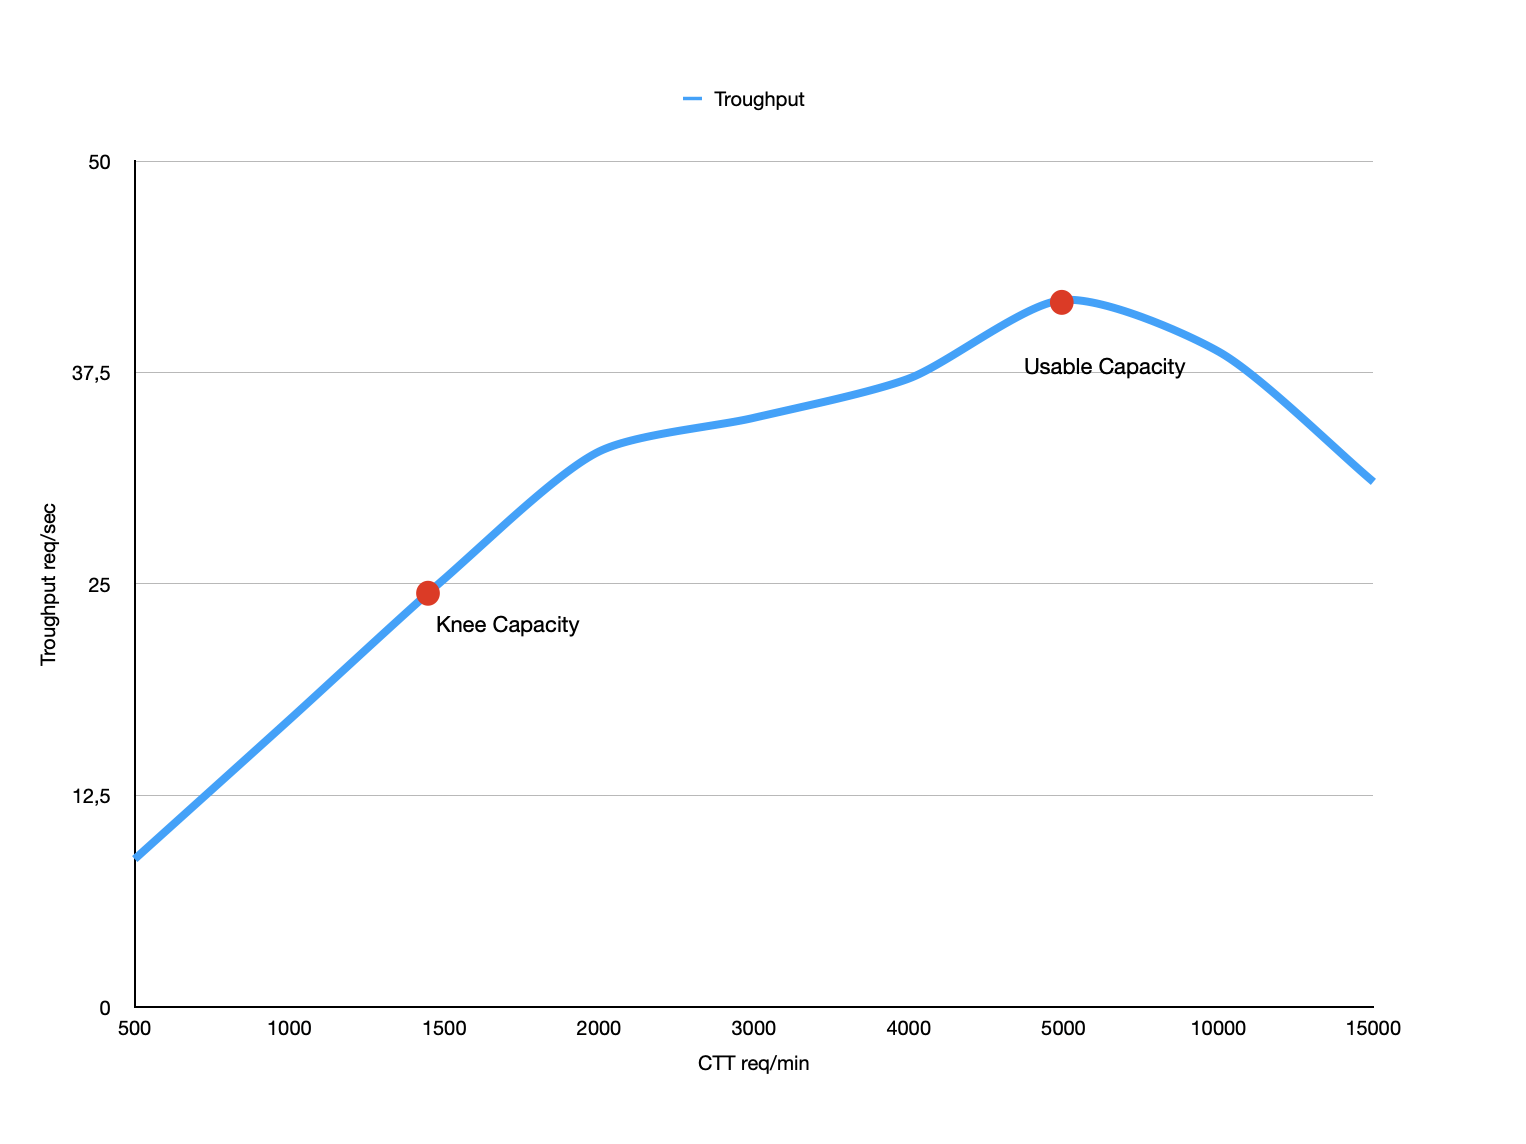
\includegraphics[scale=0.5]{img/chap_1/Througput.png}
    \caption{Throughput}
    \label{fig:thrugh}
\end{figure}
\begin{figure}[H]
    \centering
    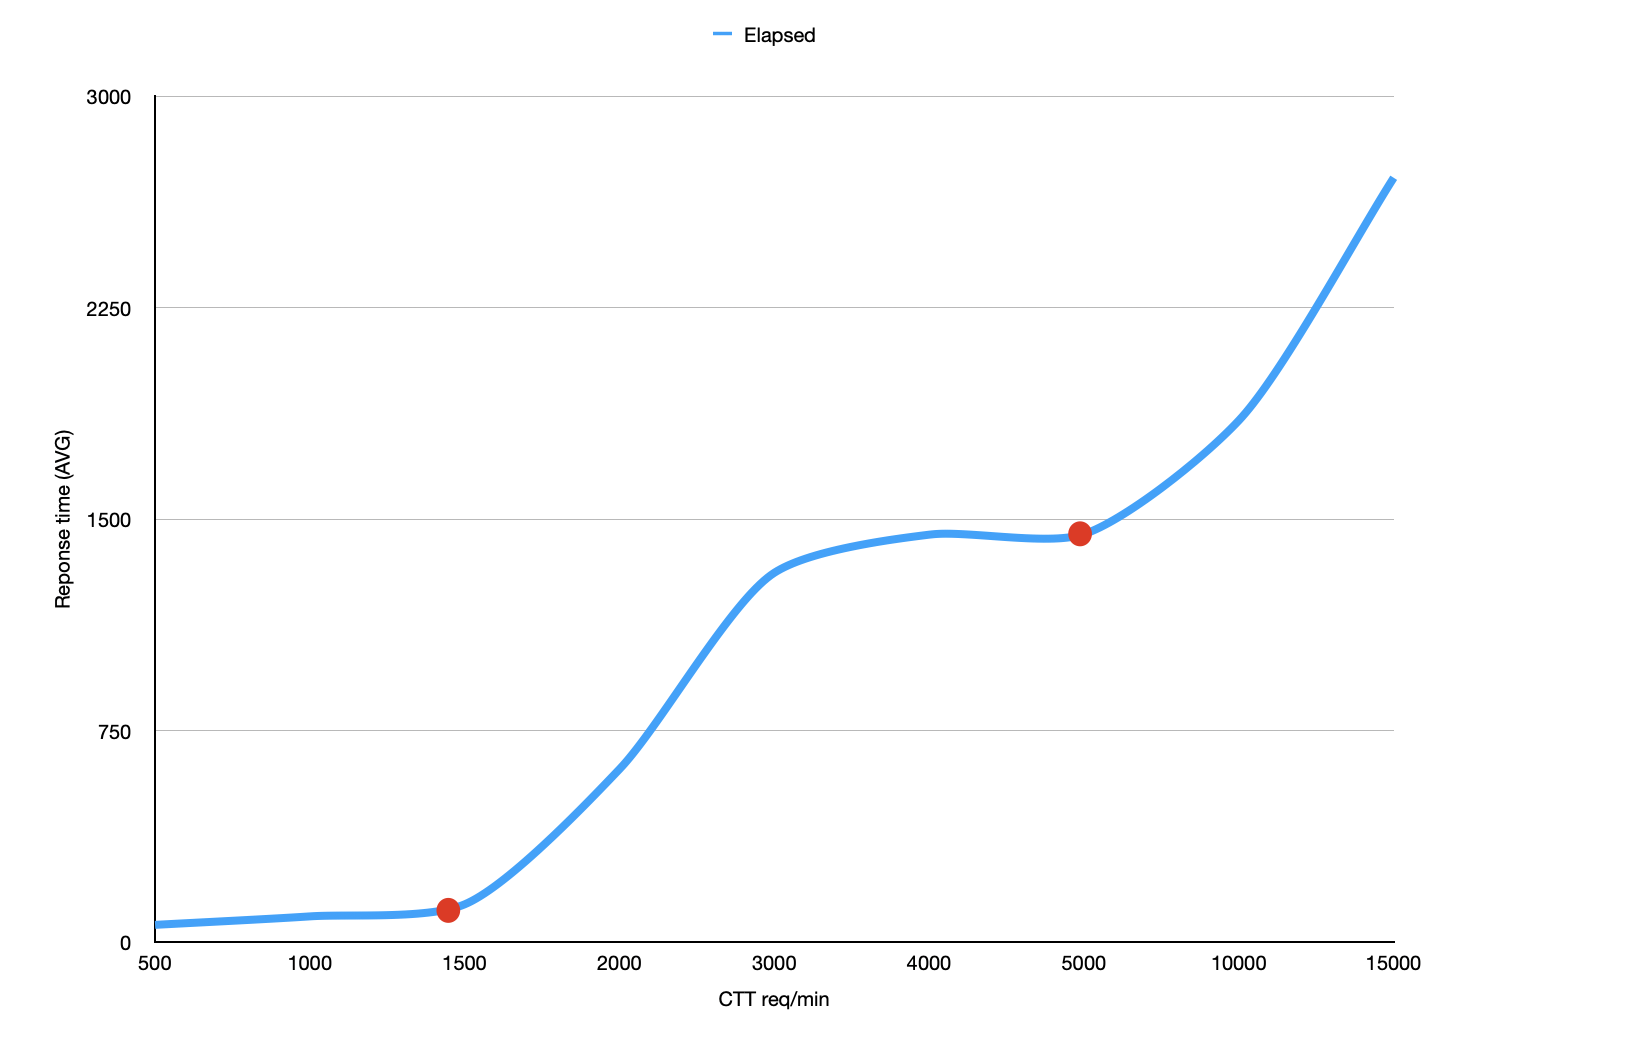
\includegraphics[scale=0.5]{img/chap_1/Response.png}
    \caption{Response}
    \label{fig:response}
\end{figure}
\begin{figure}[H]
    \centering
    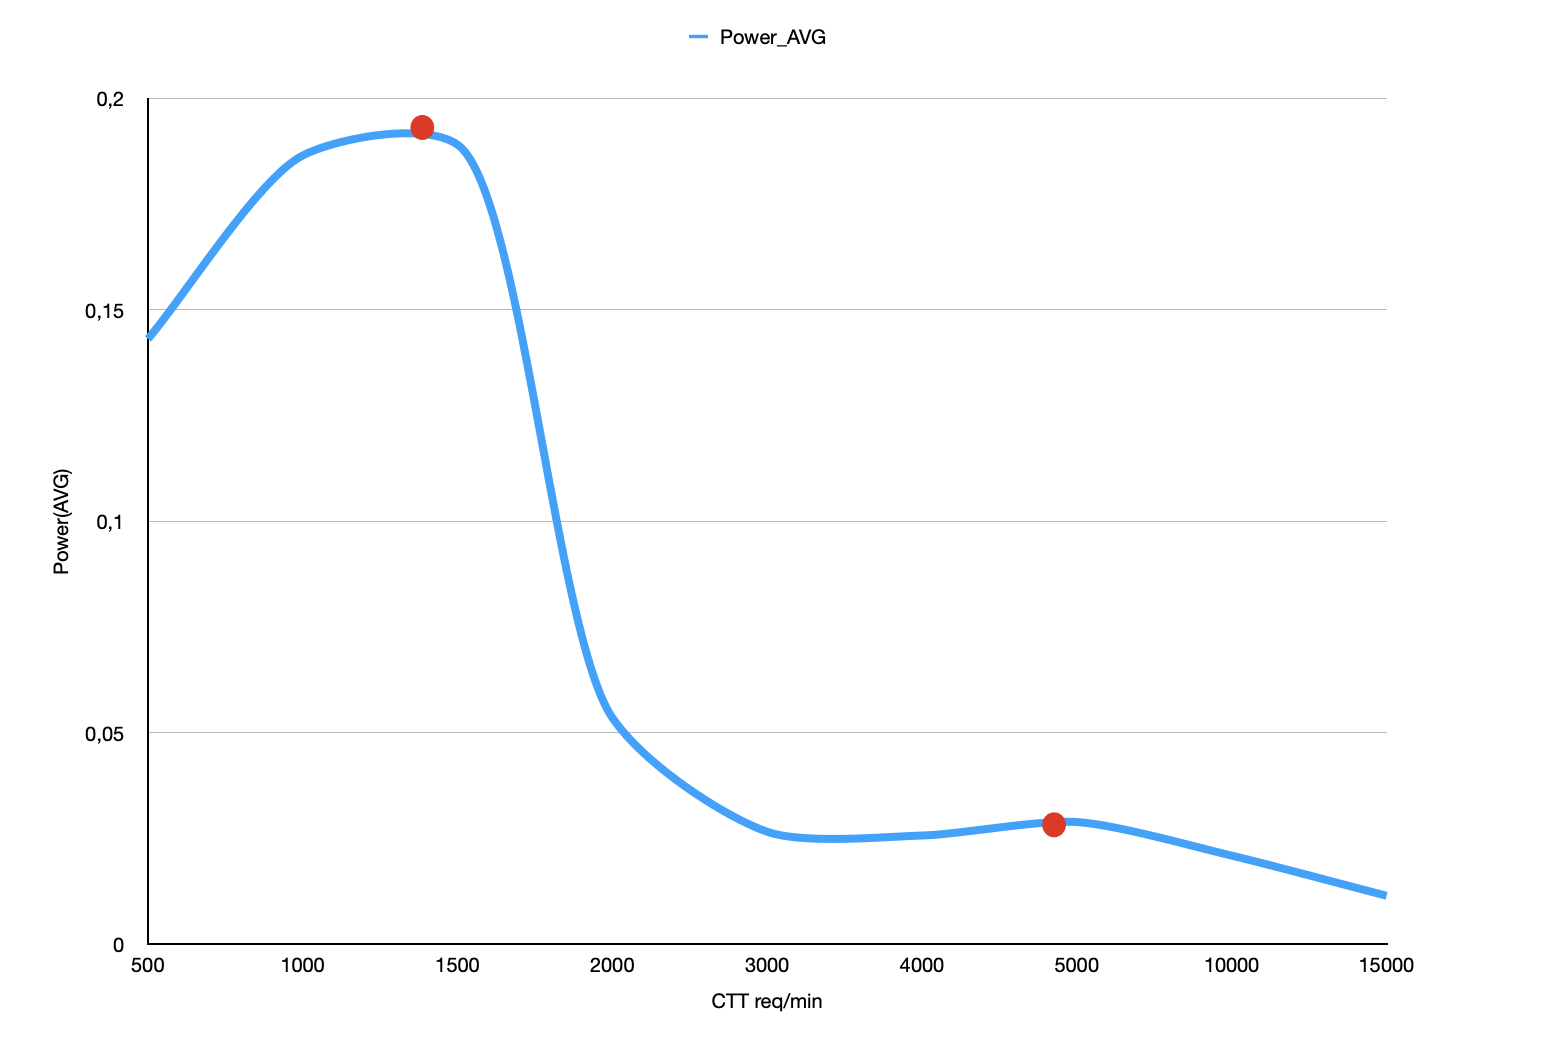
\includegraphics[scale=0.5]{img/chap_1/Power.png}
    \caption{Power}
    \label{fig:power}
\end{figure}
Dai grafici ricavai individuiamo facilmente \textit{Knee Capacity} e \textit{Usable Capacity}:
\begin{itemize}
    \item \textbf{Knee Capacity}: circa 25 req/sec con un carico di 1500 req/min
    \item \textbf{Usable Capacity}: circa 39 req/sec con un carico di 5000 req/min
\end{itemize}
\subsection{Analisi Bottleneck}
Durande la sottomissione delle richieste sono stati analizzati anche i parametri di basso livello del SUT attraverso il tool \textbf{vmstat} con il quale è stato possibile eseguire un analisi per individuare possibile bottleneck del sistema.\\
Ricordiamo che il bottleneck si presenta quando la capacità di esecuzione di un applicazione o computer è limitata da un singolo componente. Il bottleneck è la parte che presenta il mior throughput di tutte le parti. 
Anche in questa fase sono stati calcolati indici come media e coefficiente di variazione per definire se fosse meglio usare la media o la mediana e dai dati raccolti si è ritenuto opportuno usare la media.\\
Dalle analisi risulta che il sistema CPU presenta un bottleneck poichè il parametro \textbf{id}, che secondo la documentazione vmstat rappresenta la percentuale di tempo in idle, è quasi perennemente allo 0\% come dimostrato dal successivo grafico.
\begin{figure}[H]
    \centering
    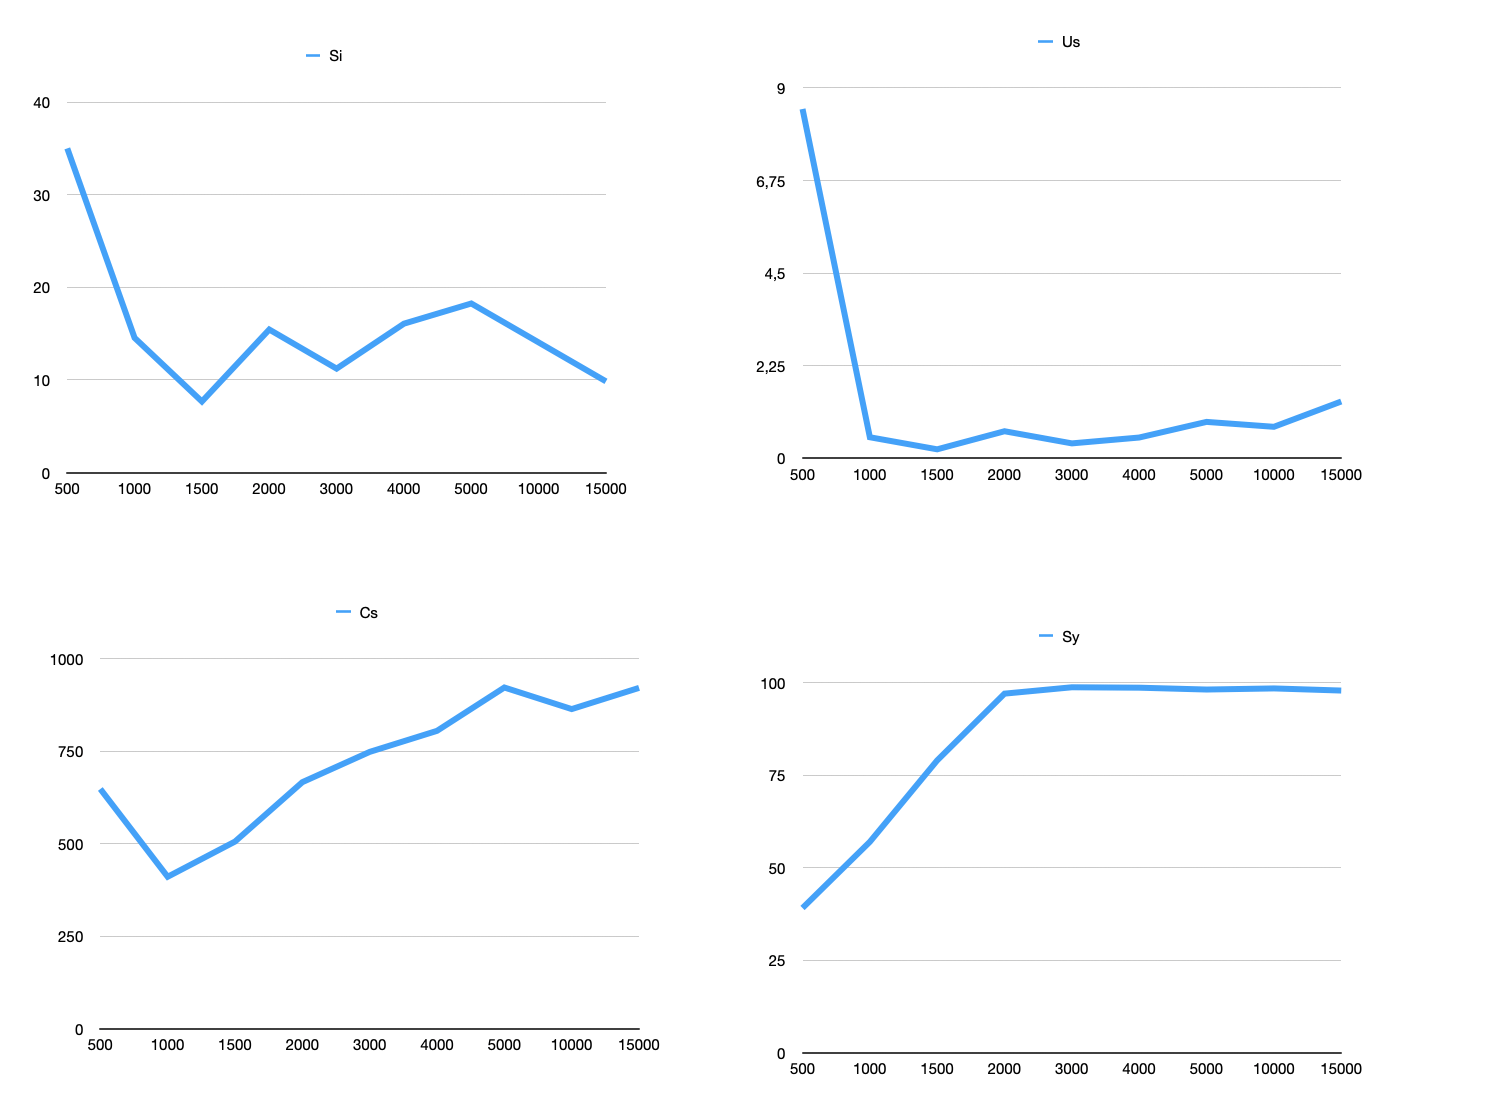
\includegraphics[scale=0.5]{img/chap_1/Bottleneck.png}
    \caption{Parametri CPU vmstat}
    \label{fig:bottleneck}
\end{figure}
\noindent
Per provare la significatività dei risultati si è deciso di effettuare un DoE one factor con 3 ripetizioni in modo da stimare l'errore.\\
Avendo raccolto i dati necessari è stato valutato il modello come si può osservare di seguito.
\begin{figure}[H]
    \centering
    \includegraphics[scale=0.5]{img/chap_1/DoEBottleneck.png}
    \caption{Modello DoE Bottleneck}
    \label{fig:doeBott}
\end{figure}
\noindent
Come si può osservare dalla figura \ref{fig:doeBott} possiamo osservare che SSE = $\frac{1998,886}{11744,525}$ = 17\%.\\
Inoltre si è proceduto ad una analisi di significativià.\\
\begin{figure}[H]
    \centering
    \includegraphics[scale=0.5]{img/chap_1/ResiduiNonNormali.png}
    \includegraphics[scale=0.5]{img/chap_1/ShWiRes.png}
    \caption{Normalita residui}
    \label{fig:normRes}
\end{figure}
\noindent
Come si può notare dalla figura \ref{fig:normRes} i residui non sono normali, dunque bisogna usare un test non parametrico come quello di Wilcoxon che dopo averlo effettuato ha dato il seguente risultato.
\begin{figure}[H]
    \centering
    \includegraphics[scale=0.5]{img/chap_1/WilcoxonBottl.png}
    \caption{Wilcoxon Bottleneck}
    \label{fig:WilcoxBottl}
\end{figure}
\noindent
Come è possibile osservare dal test in figura \ref{fig:WilcoxBottl} abbiamo una significatività statistica e non semplice casualità.
\subsection{Indice di equità}
Tamite Apache Jmeter è stato creato un tesplan con 3 thread-group che richiedono in modo concorrente allo stesso Web Server le 9 risorse disposte.\\
Attraverso i CTT di questi thread group sono stati definiti i seguenti fair throughput:
\begin{itemize}
    \item Thread group 1: 800 req/min
    \item Thread group 2: 300 req/min
    \item Thread group 3: 400 req/min
\end{itemize}
Attraverso il summary report sono stati misurati i seguenti throughput:

\begin{itemize}
    \item Thread group 1: 372 req/min
    \item Thread group 2: 240 req/min
    \item Thread group 3: 252 req/min
\end{itemize}

I throughput normalizzati $x_{i}$ dati dal rapporto tra throughput misurati e fair sono: 
\begin{itemize}
    \item Thread group 1: 0,465
    \item Thread group 2: 0,8
    \item Thread group 3: 0,63
\end{itemize}
Avendo questi elementi possiamo calcolare l'indice di equità: 
\begin{center}
F\_I= $\frac{(\sum^n_{i=1}{x_i})^2}{n\sum^n_{i=1} (x_i)^2}$     
\end{center}
Allora avrò: 
\begin{center}
   F\_I =  $\frac{(0,465+0,8+0,63)^2}{3(0,465^2+0,8^2+0,63^2)} = \frac{3,591}{3,759}$ = 0,955
\end{center}
Si può notare che il server ha un ottimo indice di Fariness, in particolare osserviamo che è molto fair con il Thread group 2 che prevede il CTT più basso mentra è meno fair nei confronti dal primo thread group.
\section{Workload Characterization}
La workload characterization ha come obiettivo quelli di produrre un modello in grado di catturare il comportamento statico e dinamico di un carico reale cui è soggetto il \textit{System Under Test} (SUT) che sia facile da riprodurre, ripetibile e accurato.\\
La workload characterization effettuata ha come soggetto il web-server discusso in tale capitolo ed è stata sviluppata tramite le seguenti fasi:
\begin{itemize}
    \item definizione del SUT 
    \item definizione di un workload di alto livello reale applicabile al sistema.
    \item raccolta di parametri di alto e basso livello.
    \item caratterizzazione del workload di alto livello, di basso livello e generazione di un workload sintetico di alto livello.
    \item validazione del workload sintetico generato tramite il confronto statistico tra i workload di basso livello caratterizzati.
\end{itemize}
Il processo è descritto dalla seguente figura
\begin{figure}[H]
    \centering
    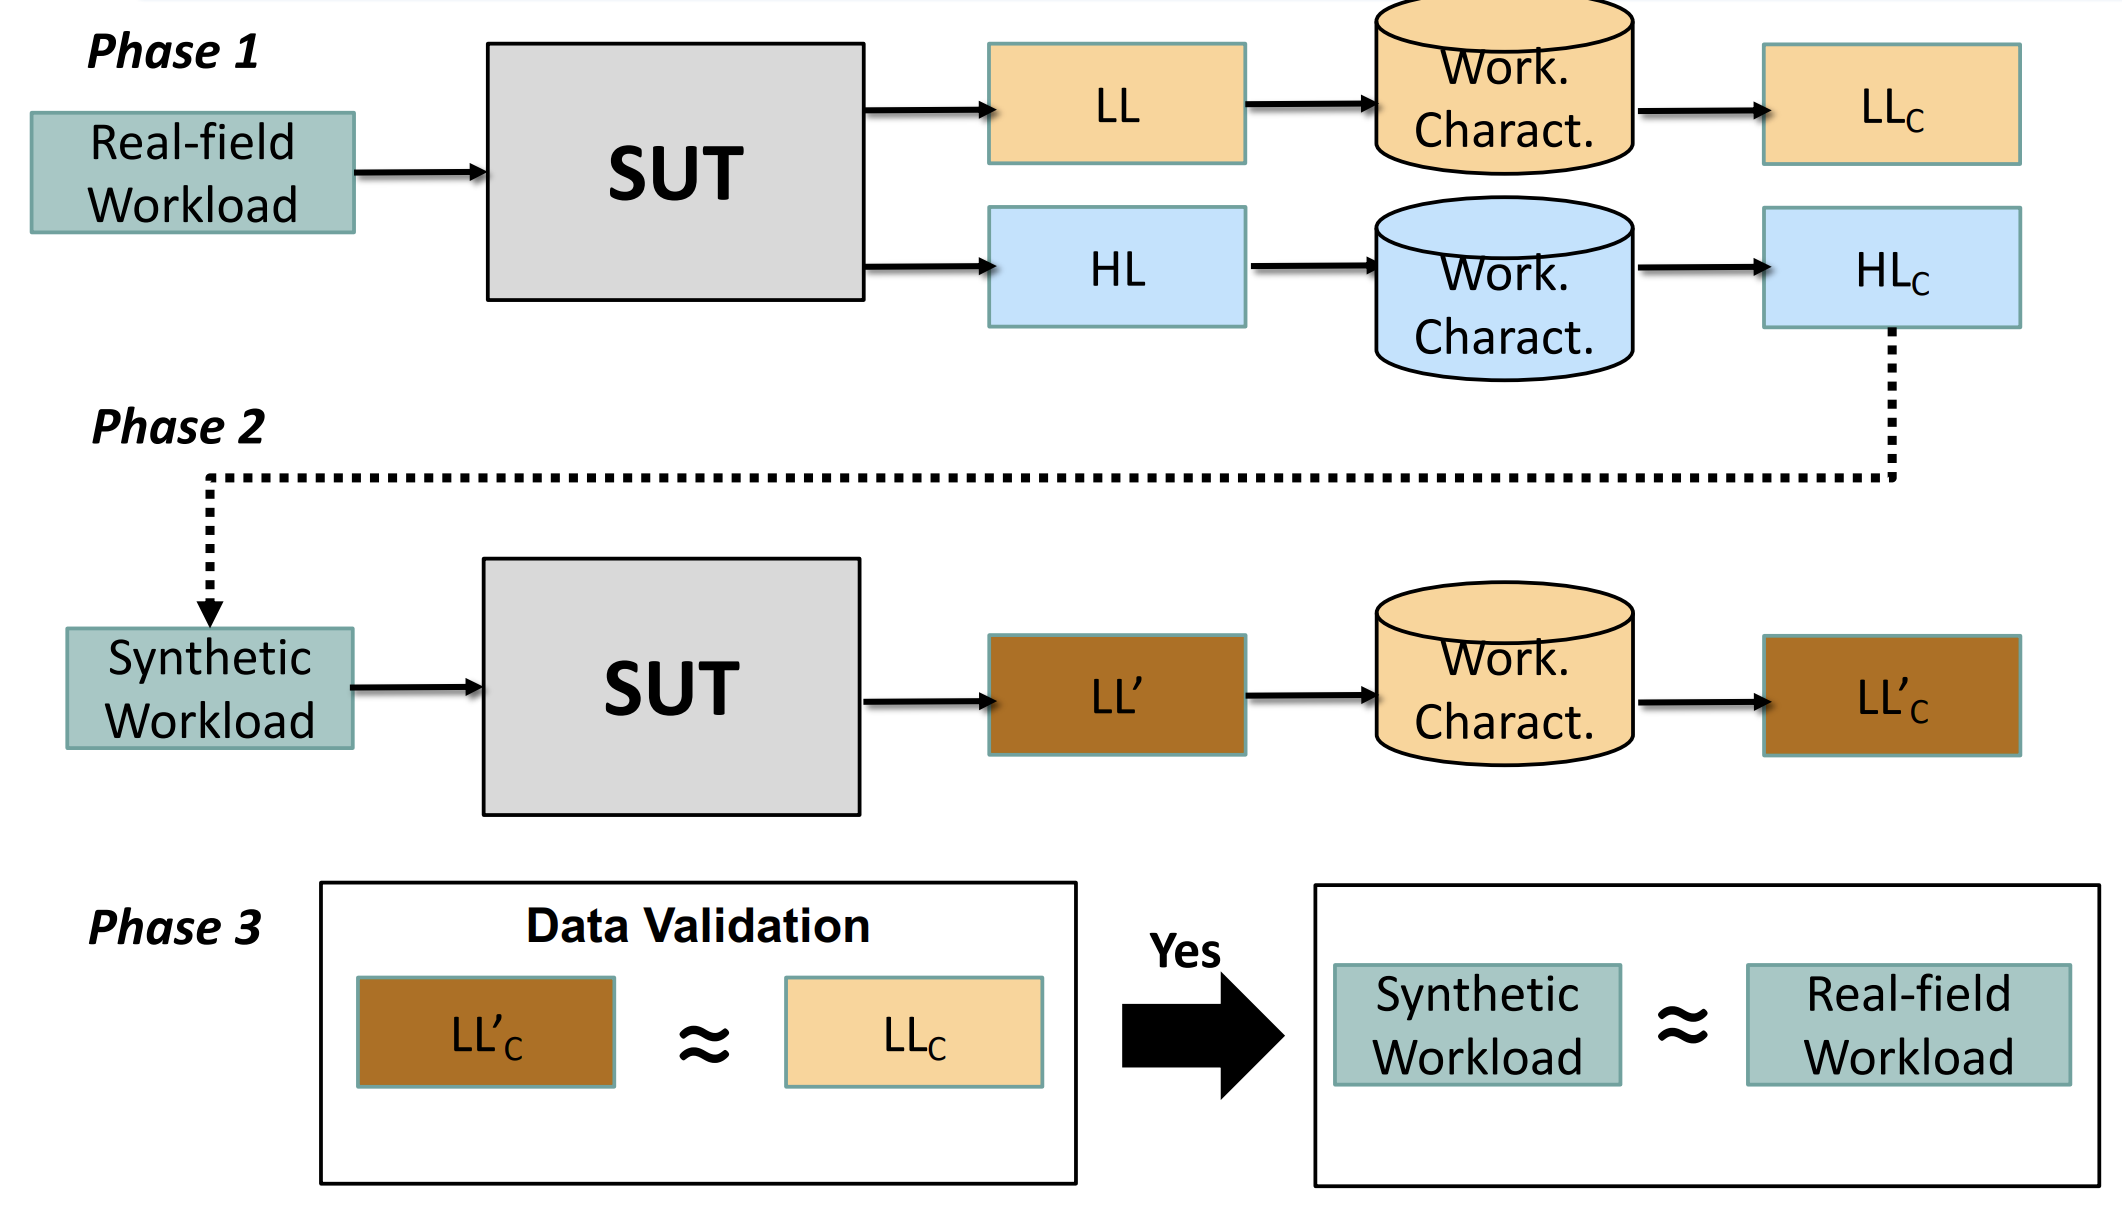
\includegraphics[scale=0.3]{img/chap_1/workLoadCharct.png}
    \caption{Processo di Workload Characterization}
    \label{fig:workLC}
\end{figure}
\subsection{Definizione del SUT}
Il Systema Under Test è un webserver Apache2 in esecuzione su macchina virtuale Oracle Virtual Box.\\
Per eseguire la workload characterization il server è stato provvisto di 40 risorse di dimensioni che variano da 1 KB fino a 20 MB con un passo di 525 KB.\\
Il workload reale di alto livello è stato generato tramite il tool JMeter.\\
Il settaggio del Test plan è il seguente:
\begin{itemize}
    \item 2 Thread Group da 20 Thread ciascuno caratterizzati da un Random Controller e un request rate di 1300 req/min.
    \item ramp up period di 1s.
    \item tempo di esecuzione dei threadgroup pari a 300s l'uno
\end{itemize}
I dati sono stati collezionati tramite un Simple Data Writer e analizzati tramite JMP.\\
Lato server, i parametri sono stati raccolti tramite il tool vmstat e anche loro analizzati con JMP.
\subsection{HL Workload Characterization}
I dati di alto livello raccolti sono stati importati su JMP ed è stata fatta una prima analisi su media e deviazione standard dei prametri.\\
Di seguito riportiamo la taberlla riassuntiva:
\begin{figure}[H]
    \centering
    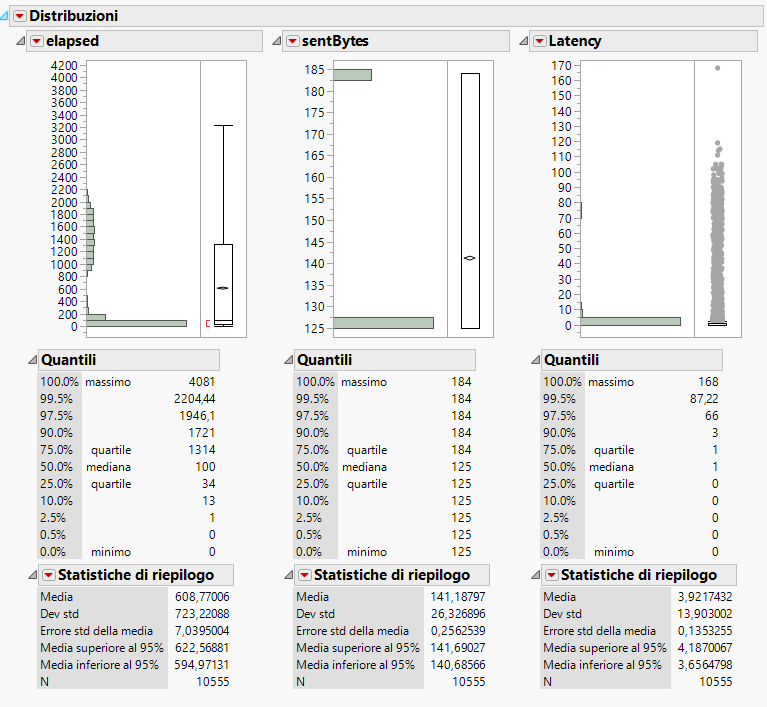
\includegraphics[scale=0.6]{img/chap_1/DistParam_hl.png}
    \caption{Tabella statistiche}
    \label{fig:stats_hl}
\end{figure}
\noindent
Come è possibile osservare dalla tabella \ref{fig:stats_hl} sia \textbf{Sample Count} che \textbf{Error Count} possono essere non considerate come colonne.\\
Una seconda analisi ha interessato le righe.\\
In particolare si è analizzata la presenza o meno di outliers solo per le colonne ritenute utili per l'analisi.\\
\begin{figure}[H]
    \centering
    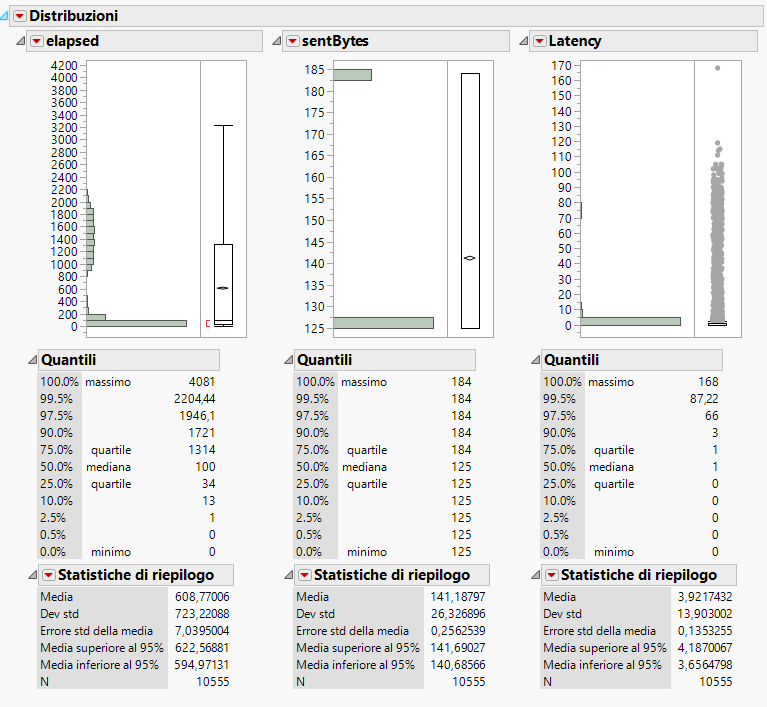
\includegraphics[scale=0.6]{img/chap_1/DistParam_hl.png}
    \caption{Distribuzione dei parametri}
    \label{fig:dist_param}
\end{figure}
\noindent
In tale analisi si è deciso di non filtrare righe poichè non vi sono particolari outliers.\\
Dopodichè è stata eseguita la PCA che riportiamo di seguito:
\begin{figure}[H]
    \centering
    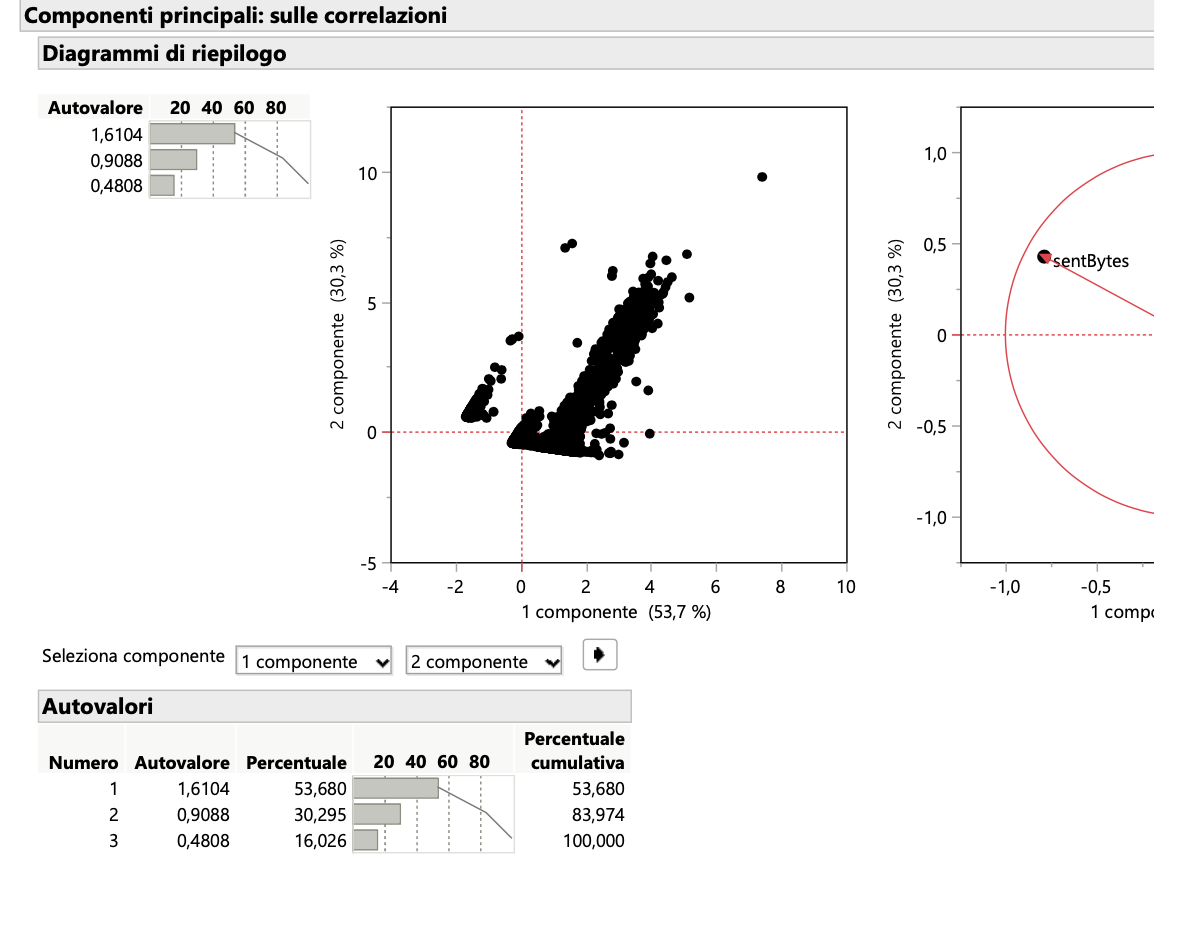
\includegraphics[scale=0.3]{img/chap_1/PCA_HL.png}
    \caption{Clustering HL}
    \label{fig:clust_hl}
\end{figure}
\noindent
Poichè la dimensionalità è molto esigua  si è proceduto a selezionare tutte le componenti principali.\\
Dopo aver effettuato la PCA è stato effettuato il Clustering.\\
Di seguito riportiamo la procedura che JMP ha eseguito 
\begin{figure}[H]
    \centering
    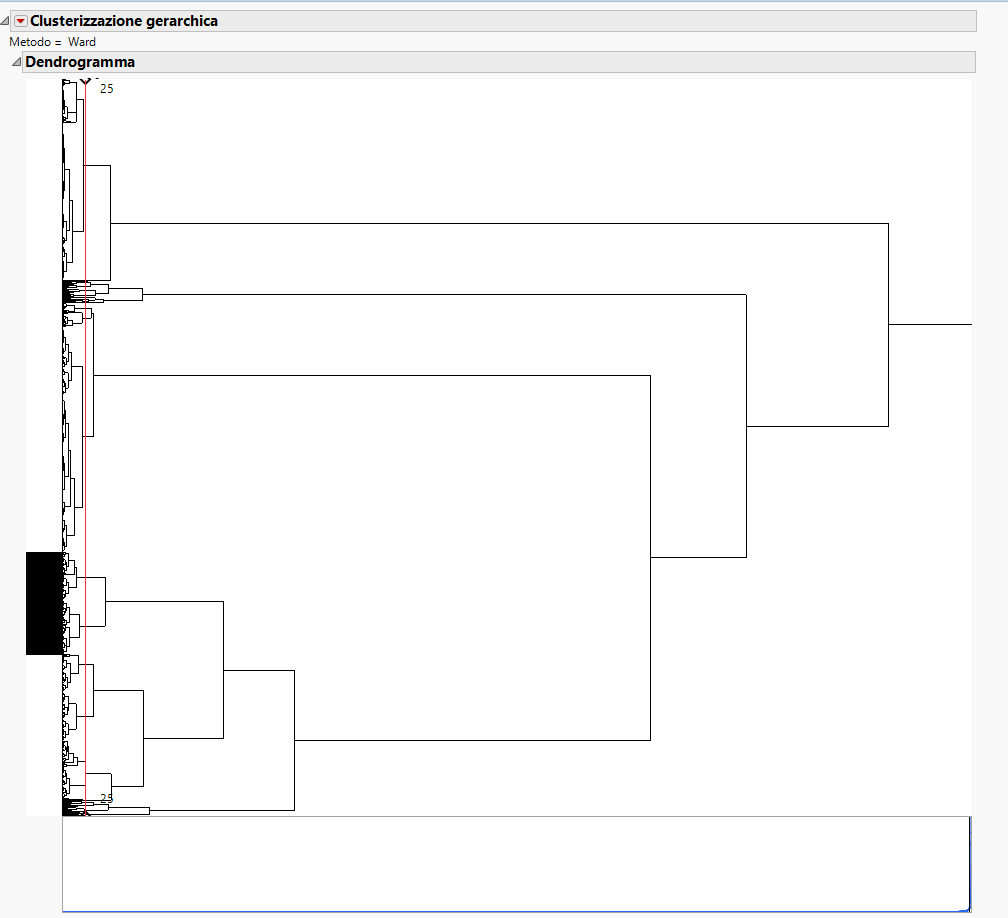
\includegraphics[scale=0.3]{img/chap_1/ClustHL.png}
    \caption{Clustering HL}
    \label{fig:clust_hl}
\end{figure}
\noindent
Osservando la figura in basso al dendogramma abbiamo concluso che il miglior numero di cluster che potevamo contemplare fosse 25 con una perdita dello 0.008\%.\\
\begin{figure}[H]
    \centering
    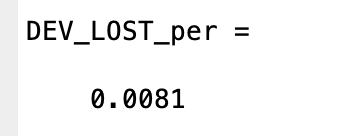
\includegraphics[scale=0.5]{img/chap_1/var_loss_hl.png}
    \caption{Clustering HL}
    \label{fig:clust_hl}
\end{figure}
\noindent
Per scegliere le richieste HTTP si è svolta una analisi di contingenza del parametro label rispetto al cluster attraverso uno script python che seleziona la richiesta più rappresentativa di un determinato cluster (attraverso un approccio frequentista) e la eliminava dal dataset (per evitare che comparisse come richiesta rappresentativa anche di un cluster diverso).\\
Di seguito riportiamo la scelta effettuata dallo script:
\begin{figure}[H]
    \centering
    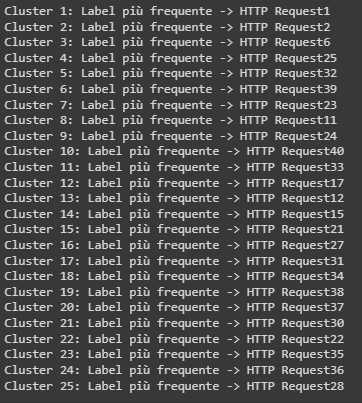
\includegraphics[scale=0.5]{img/chap_1/ChoiceHL.png}
    \caption{Scelta richieste HTTP}
    \label{fig:ch_http_req}
\end{figure}
\noindent
Tale scelta rappresenta anche il Workload sintetico che va riapplicato al SUT.
\subsection{LL Workload Characterization}
La caratterizzazione di basso livello che come obiettivo quello di estrarre punti rappresentativi dei componenti principali con una certa percentuale di varianza spiegata in modo da poterle confrontare con quelle del workload di basso livello ottenuto a seguito dell'applicazione del workload sintetico di alto livello.\\
Anche qui i dati sono stati importati su JMP ed è stata effettuata una analisi su media e deviazione standard.\\
Di seguito riportiamo la tabella riassuntiva:
\begin{figure}[H]
    \centering
    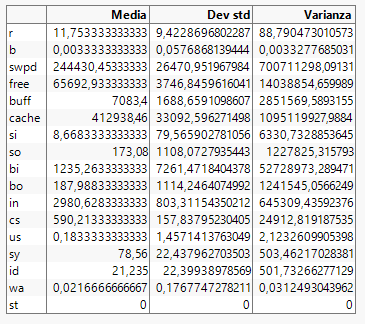
\includegraphics[scale=0.6]{img/chap_1/stats_param_ll1.png}
    \caption{Statistiche LL}
    \label{fig:ll_stats}
\end{figure}
\noindent
Come si può vedere dalla tabella \ref{fig:ll_stats} la colonna \textbf{st} può essere esclusa dalle successive analisi.\\
Anche per questo dataset è stata fatta una analisi sulla distribuzione, ma anche in questo caso non è stato necessario apportare un filtraggio sulle righe del dataset.\\
Si è passati dunque all'analisi multivariata attraverso la PCA che possiamo vedere dalle seguenti figure:
\begin{figure}[H]
    \centering
    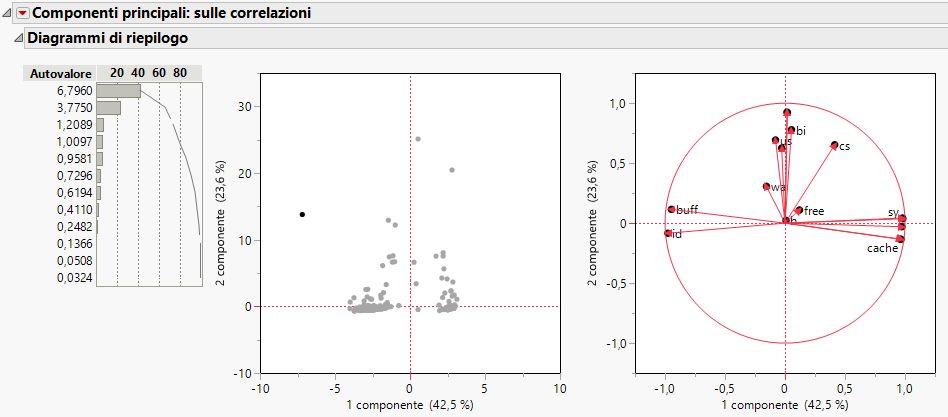
\includegraphics[scale=0.6]{img/chap_1/PCA_1.png}
    \caption{PCA parametri LL}
    \label{fig:pca_ll}
\end{figure}
\noindent
\begin{figure}[H]
    \centering
    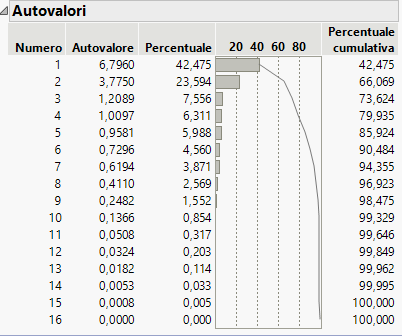
\includegraphics[scale=0.6]{img/chap_1/Autovalori_1.PNG}
    \caption{Autovalori PCA LL}
    \label{fig:autoval_ll}
\end{figure}
\noindent
Dall'analisi multivariata della PCA si è deciso di preservare il 94\% della varianza circa e quindi di selezionare 7 componenti principali.\\
Dopo la procedura di riduzione della dimensionalità delle colonne si è passati al clustering.\\
\begin{figure}[H]
    \centering
    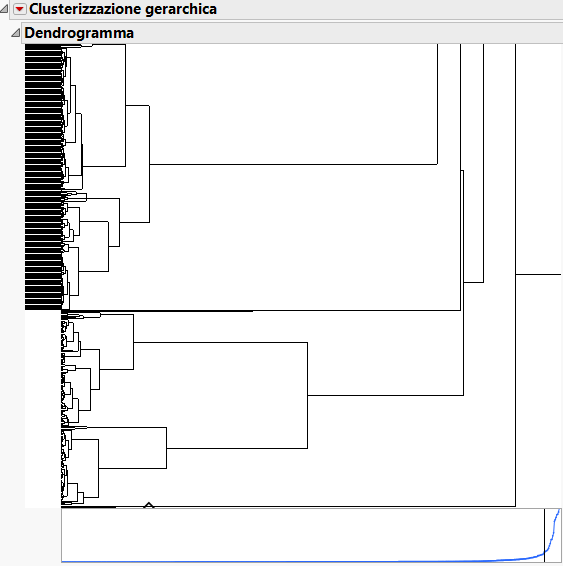
\includegraphics[scale=0.6]{img/chap_1/Clust_1.PNG}
    \caption{Clustering LL}
    \label{fig:clust_ll}
\end{figure}
\noindent
Sempre facendo riferimento al grafico in basso al dendogramma sono stati scelti 20 cluster.\\
Tale scelta ha portato alla perdita di un ulteriore 9\% di varianza.\\
\begin{figure}[H]
    \centering
    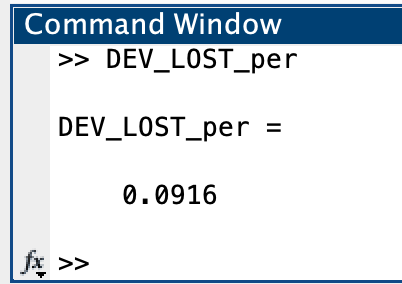
\includegraphics[scale=0.6]{img/chap_1/Varianza_persa_clustering.PNG}
    \caption{Varianza persa LL}
    \label{fig:variance_loss}
\end{figure}
\noindent
Anche in questo caso sono stati scelti tanti parametri quanti sono i cluster, dunque 20.\\
La scelta è stata fatta attraverso uno script Python che ha scelto in maniera randomica i parametri da prendere in considerazione per ogni cluster, producendo il seguente dataset:
\begin{figure}[H]
    \centering
    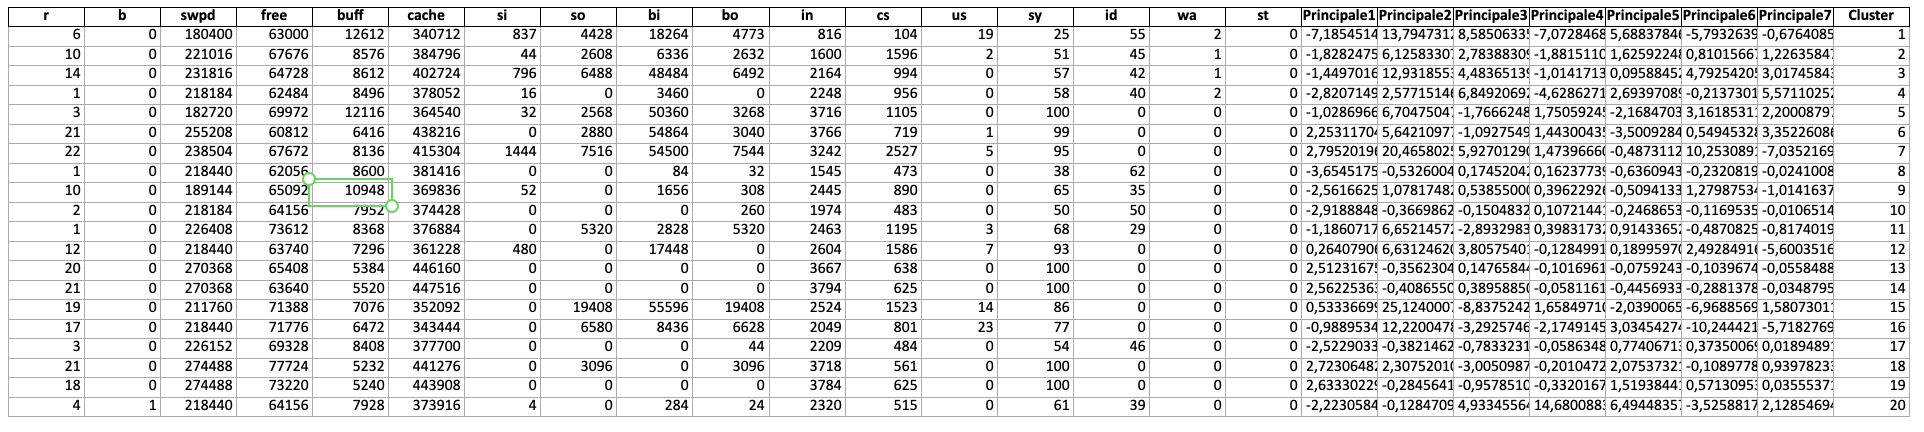
\includegraphics[scale=0.4]{img/chap_1/ll_dataset.png}
    \caption{Dataset LL}
    \label{fig:data_selected_LL}
\end{figure}
\noindent
\subsection{LL' Workload Characterization}
Dopo aver stilato il Workload sintetico, sono state inibite le richieste che non appaiono in quest'ultimo su Jmeter e si è risottoposto il server a questo workload.\\
La sottomissione di questo workload ha prodotto altre statistiche di basso livello di cui si è effettuata l'analisi.\\
In questo caso anche si è effettuata una analisi su media e deviazione standard che però hanno evidenziato ancora che il parametro st non influisca sui dati poichè ha varianza e media nulla.\\
Anche l'analisi sulla distribuzione non ha evidenziato perticolari dati da cancellare.\\
Anche su questi dati è stata effettuata la stessa analisi effettuata per il dataset LL del workload reale, in particolare sono state prese le stesse componenti principali (7) e gli stessi cluster (20) per permettere il confronto statistico tra i due dataset.\\
\subsection{Confronto tra workload}
Per effettuare un confronto statistico dei campioni significativi dei componenti principali , è stata effettuate le seguente considerazione:
\begin{itemize}
    \item \textbf{Verifica di normalità dei campioni}: tale verifica è stata effettuata per capire se è possibile effettuare un test parametrico o non parametrico.\\
    Non abbiamo un numero sufficiente di campioni per assicurarci la normalità secondo il TLC per cui è necessario verificare la normalità dei dati.
\end{itemize}
Di seguito riportiamo i QQ-plot riassuntivi.\\
\begin{figure}[H]
    \centering
    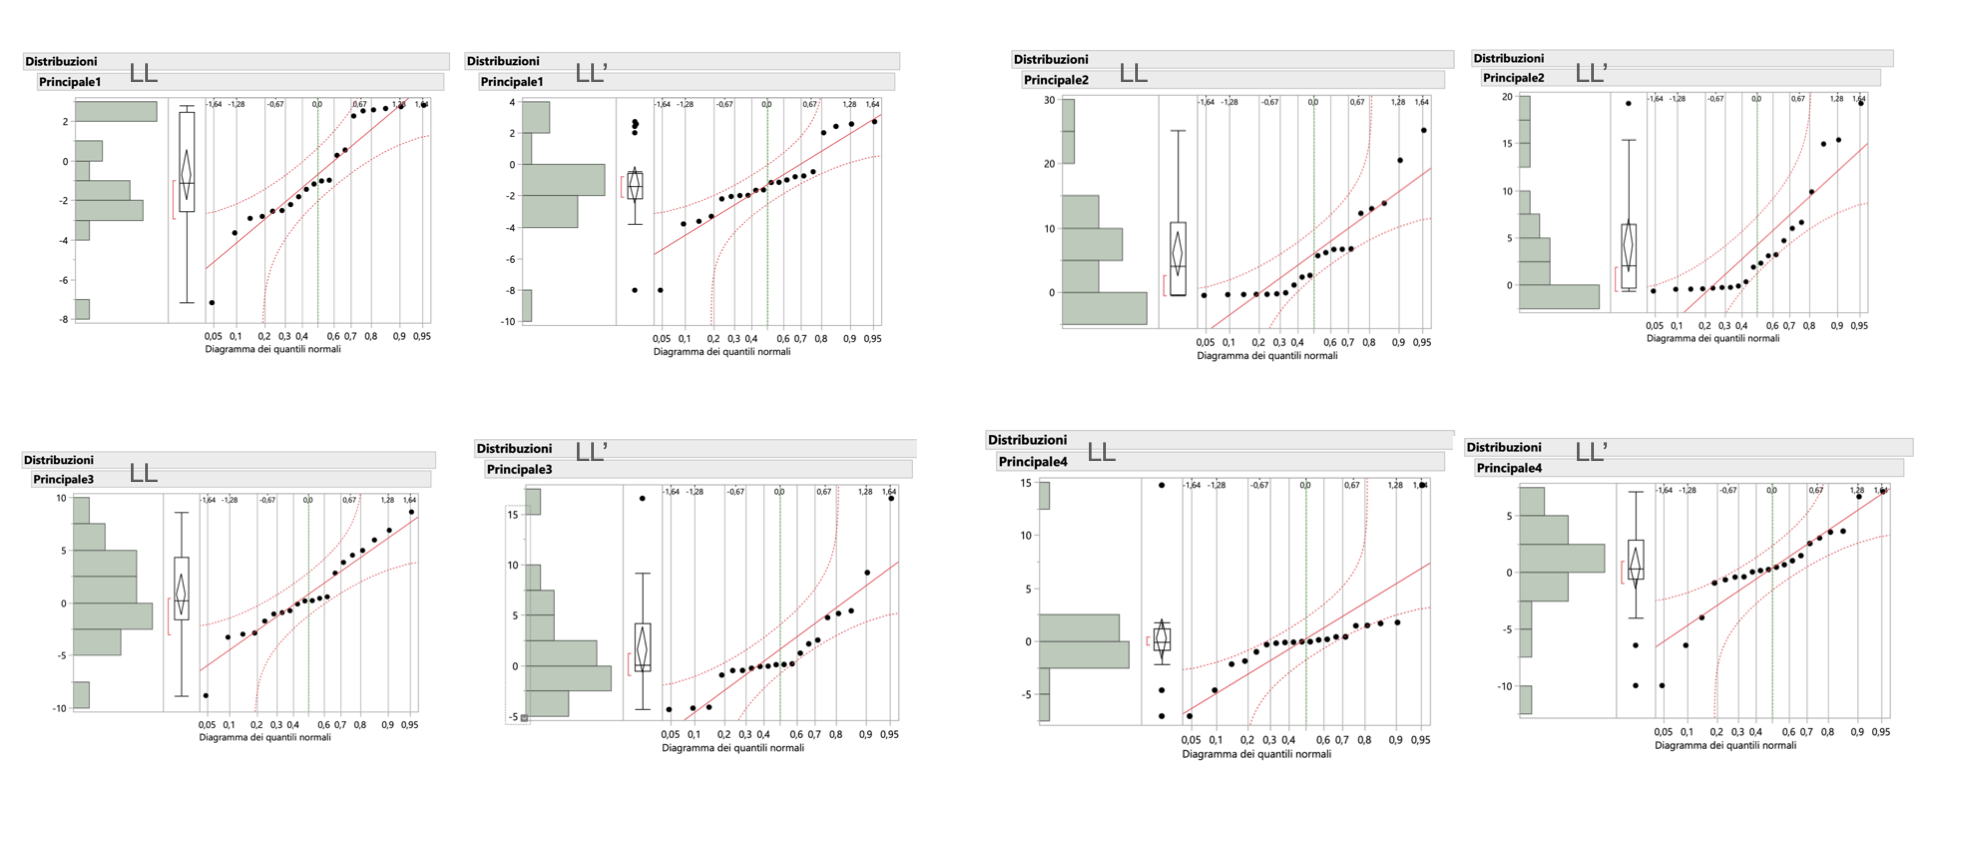
\includegraphics[scale=0.4]{img/chap_1/qq_plots1.png}
    \caption{QQ plot dati LL e LL'}
    \label{fig:qq_plot_ll1}
\end{figure}
\noindent
\begin{figure}[H]
    \centering
    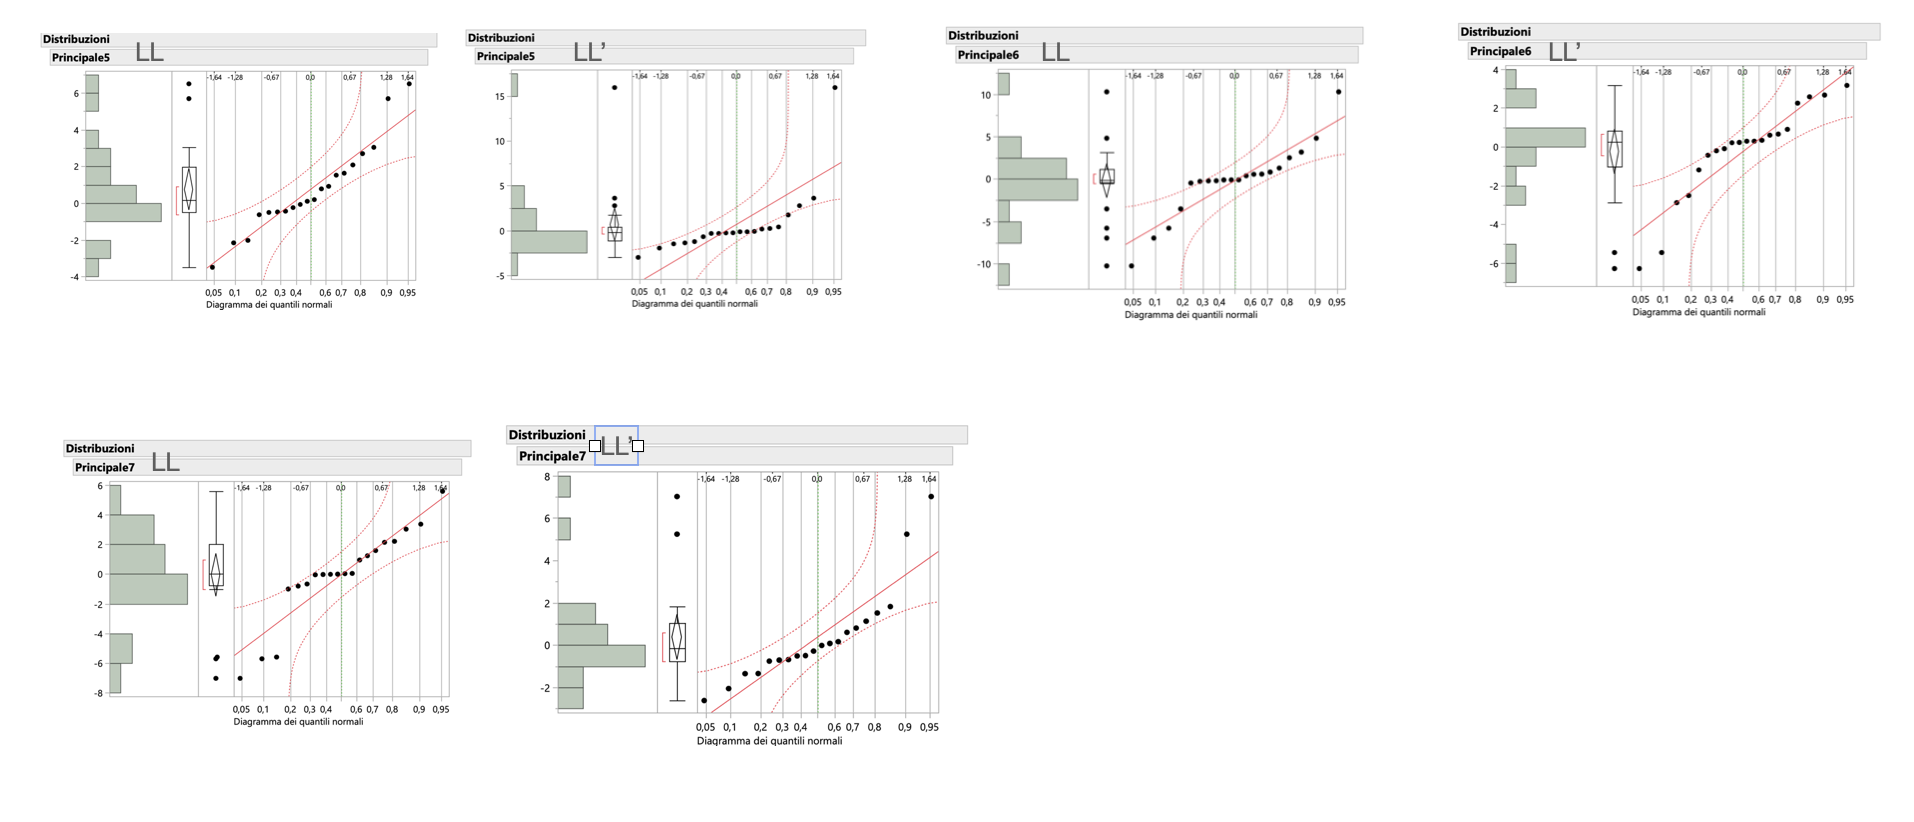
\includegraphics[scale=0.4]{img/chap_1/qq_plots2.png}
    \caption{QQ plot dati LL e LL'}
    \label{fig:qq_plot_ll2}
\end{figure}
\noindent
Dai qq-plots si è deciso di trattare come distribuzioni normali e quindi con test parametrici le componenti principali \textbf{1} e \textbf{7} mentre tutte le altre verranno trattate con test non parametrici.\\
Per queste ultime si è usato il test di Wilcoxon (ranksum su Matlab) di cui riportiamo una tabella con risultato del test e valore del p-value.
\begin{table}[htbp]
    \centering
    \label{tab:esempio}
    \begin{tabular}{|c|c|c|c|} % specifica il numero e l'allineamento delle colonne (c = centrato, l = sinistra, r = destra)
        \hline
        Componente & p-value & Risultato test \\ % separa le celle con '&', e termina ogni riga con '\\'
        \hline
        2 & 0.4570 & 0 \\
        3 & 0.8181 & 0 \\
        4 & 0.3648 & 0\\
        5 & 0.4249 & 0\\
        6 & 0.8817 & 0\\
        \hline
    \end{tabular}
\end{table}
\\
Come Si può vedere la tabella per le componenti principali evidenzate non vi è differenza statistica poichè il test non riesce a rigettare l'ipotesi nulla.\\
Per le componenti 1 e 7 si è proceduto all'uso del T-Test aggregato parametrico, data la normalità dei campioni, che ha dato i seguenti risultati 
\begin{figure}[H]
    \centering
    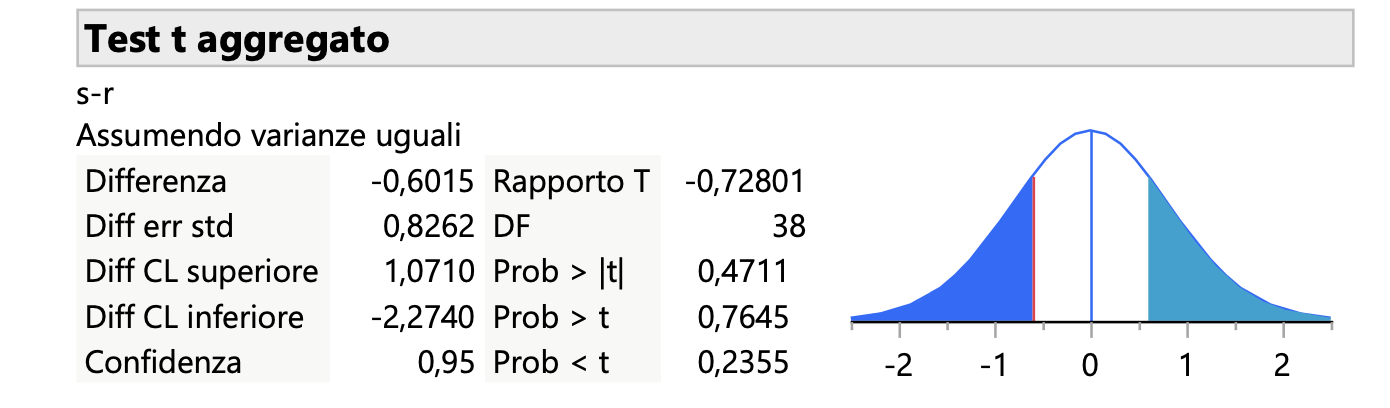
\includegraphics[scale=0.4]{img/chap_1/t_test1.png}
    \caption{T-test componente 1}
    \label{fig:t_test1}
\end{figure}
\noindent
\begin{figure}[H]
    \centering
    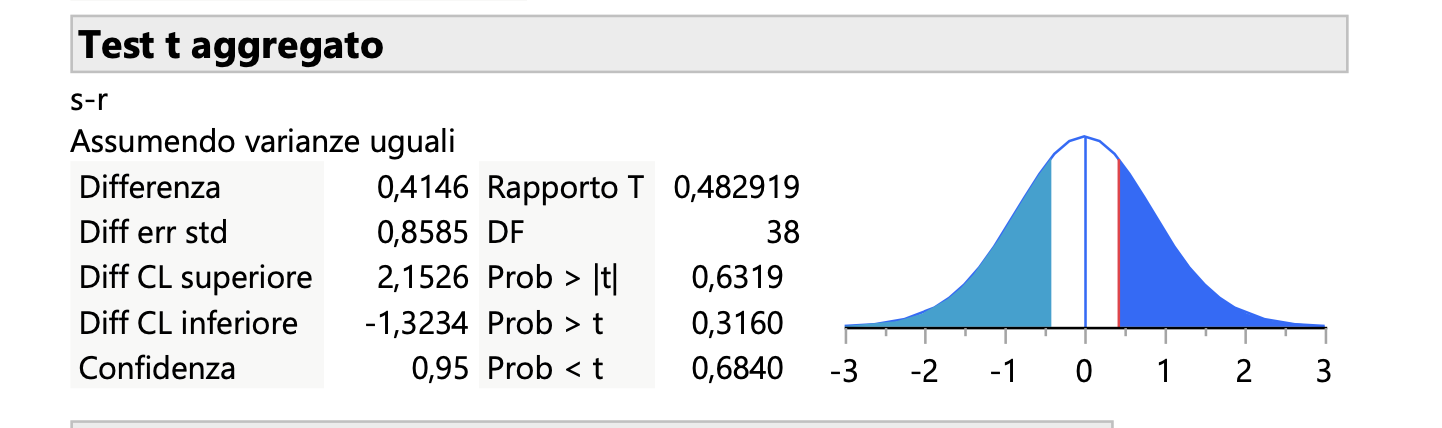
\includegraphics[scale=0.4]{img/chap_1/t_test2.png}
    \caption{T-test componente 7}
    \label{fig:t_test2}
\end{figure}
\noindent
Entrambe i test non rigettano l'ipotesi nulla e quindi con il 95\% di confidenza possiamo affermare che non vi sia differenza statistica per le popolazioni da cui sono stati estratti i campioni.
\section{DoE}
In questo paragrafo descriveremo il processo di creazione di un piano sperimentale detto \textbf{Design of experiment}.\\
Tale processo permette di determinare quali sono i fattori che più influiscono su una particolare metrica di performance misurata sul SUT.\\
Le variabili che influenzano l'uscita sono detti fattori e ad ogni fattore sono associati dei livelli, ovvero valori che il fattore può assumere.\\
Il SUT in esame è sempre il webserver di questo capitolo e le richieste al sistema saranno effettuate sempre tramite apache JMeter.\\
Per il piano attuato abbiamo:
\begin{itemize}
    \item \textbf{Intensità}: indica il carico imposto al sistema e ha 3 livelli low( 25\% della usable capacity), medium(50\% della usable capacity) e high (75\% della usable capacity).
    Dato che la usable capacity è stata individuata a 5000 req/min avrò la low a 1250 req/min, medium 2500 req/min e la high a 3750 req/min.

    \item \textbf{Page size}: dimensione della pagina richiesta al webserver. Il fattore è caratterizzato da 4 livelli small (1KB - 550 KB), medium ( 551KB - 1 MB), large (1MB - 10MB)  
\end{itemize}
Come variabile di risposta si è scelto il response time definito come il tempo che il server impiega a servire una richiesta indirizzata ad una certa risorsa con una determinata intensità e quindi è selezionato come la media degli elapsed.\\
Il numero di ripetizioni fissato per il piano è 5 ripetizioni per definire l'errrore di stima degli effetti dei fattori.\\
Il piano sperimentale è di tipo \textbf{full factorial} e questo ci porta ad eseguire $3^2 \cdot 5 = 45$ esperimenti.\\
Di seguito riportiamo gli esperimenti:
\begin{figure}[H]
    \centering
    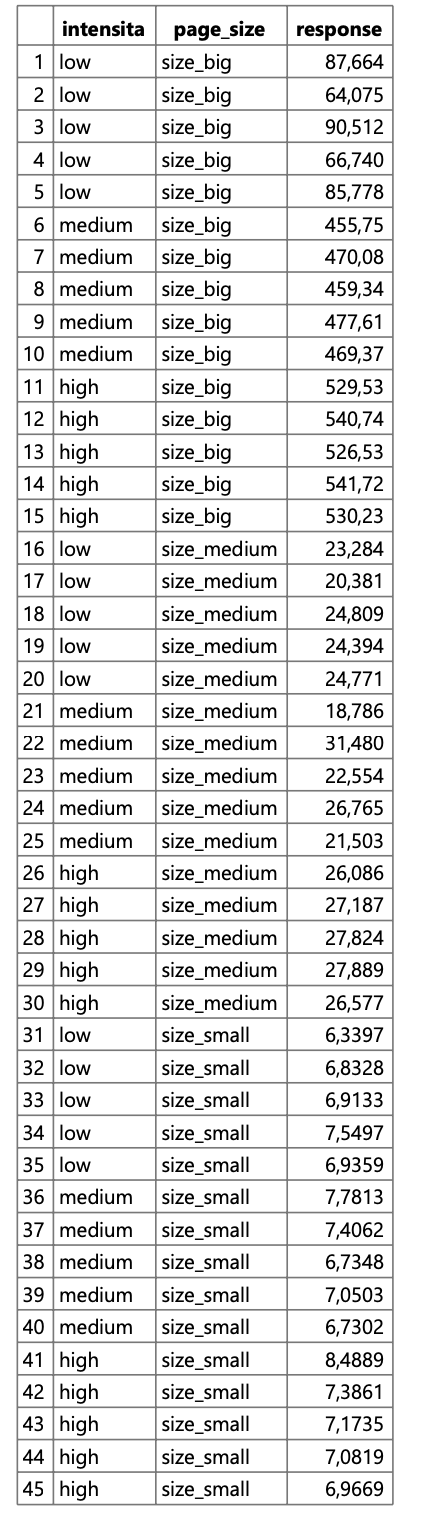
\includegraphics[scale=0.4]{img/chap_1/exp_doe.png}
    \caption{Esperimenti}
    \label{fig:exp_doe}
\end{figure}
\noindent
Una volta effettuati gli esperimenti abbiamo definito, tramite JMP, l'importanza di ogni fattore.\\
Avremo il seguente risultato:
\begin{figure}[H]
    \centering
    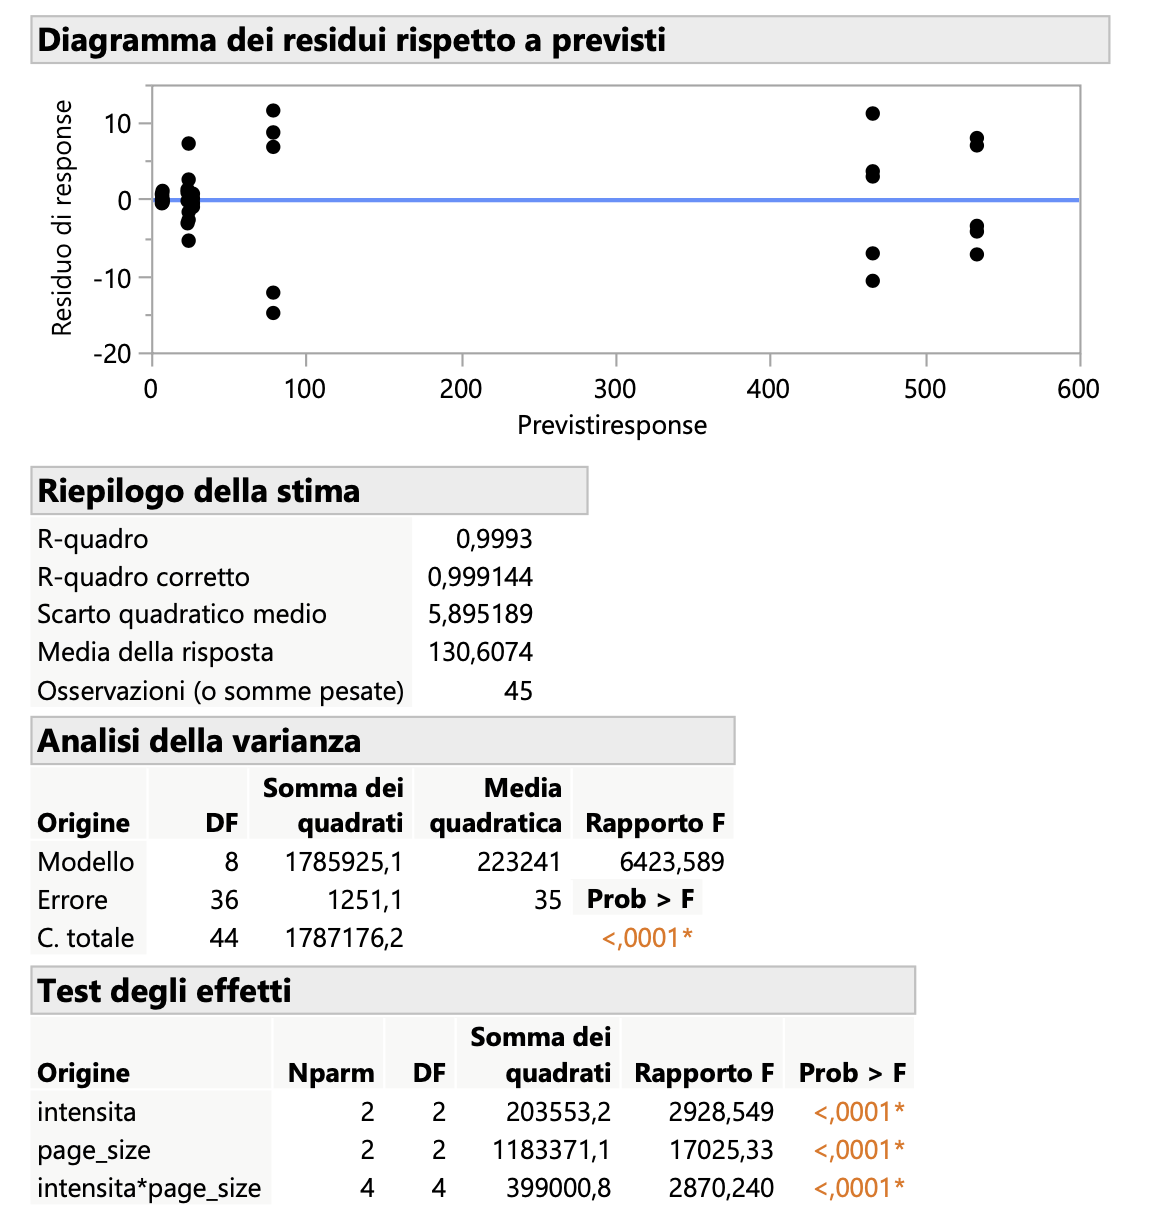
\includegraphics[scale=0.4]{img/chap_1/var_alloc.png}
    \caption{Allocazione della varianza}
    \label{fig:var_alloc}
\end{figure}
\noindent
Come si può osservare dall'analisi della varianza una grande parte della varianza è spiegata dal modello, inoltre una grande parte di quest'ultima è allocata al fattore \textit{page\_size}.\\
Possiamo definire l'importanza facendo il rapporto tra varianza allocata al fattore e quella totale.\\
Avremo dunque:
\begin{center}
    
    $\frac{SSE}{SST} = \frac{1251}{1787176,2} = 0,0006\% $\\
    $\frac{SS_{intensity}}{SST} = \frac{203553,2}{1787176,2} = 11\%$ \\
    $\frac{SS_{pageSize}}{SST} = \frac{1183371,1}{1787176,2}=66\%$ \\
    $\frac{SS_{interaction}}{SST} = \frac{399000,8}{1787176,2}=22\% $
    
\end{center}
Da questa analisi possiamo ottenere una descrizione sull'importanza dei fattori nella risposta.\\
Il fattore fondamentale come si può vedere è il \textit{page\_size} portando con se il 66\% della varianza complessiva.\\
Inoltre è importante anche l'interazione che porta con se il 22\% della varianza.\\
L'errore come si può facimente osservare risulta marginale e associato dunque ad una percentuale di varianza molto piccola.\\
Fatta una analisi sull'importanza possiamo passare ad una analisi riguardo la significativià.\\
In particolare per lo studio è stata utilizzata l'ANOVA (Analysis of Variance).\\
Ricordiamo che la \textbf{significatività} ci dice che quello che abbiamo osservato non è frutto dell'aleatorietà.\\
Per determinare quale tipo di ANOVA si è condotta una analisi sulla distribuzione dei residui, ovvero attraverso un QQ-plot si è verificato che questi residui siano normali.\\
\begin{figure}[H]
    \centering
    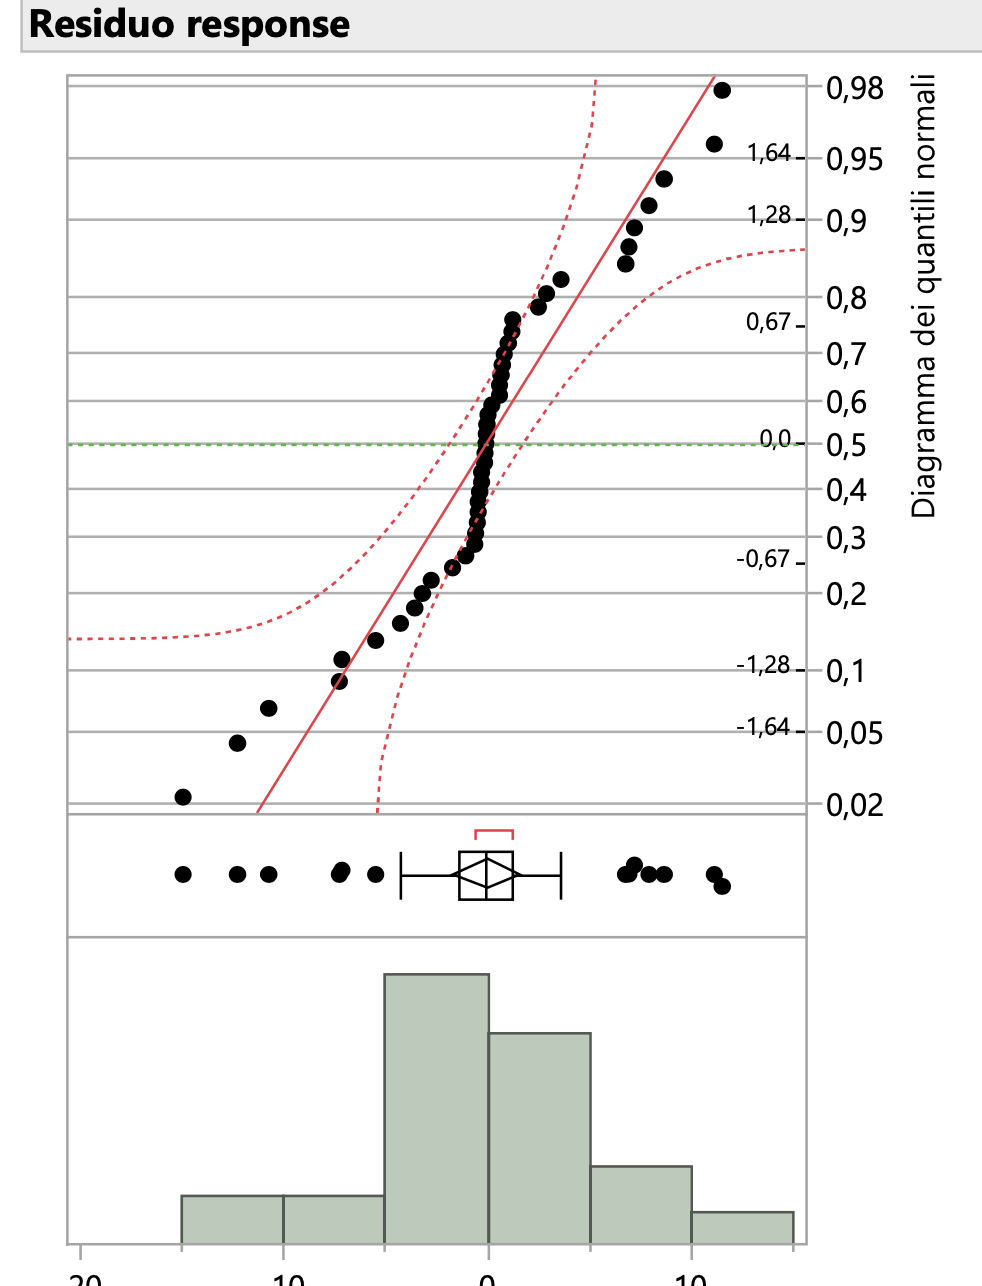
\includegraphics[scale=0.4]{img/chap_1/res_norm.png}
    \caption{qq-plot residui}
    \label{fig:qq_res_plot}
\end{figure}
\begin{figure}[H]
    \centering
    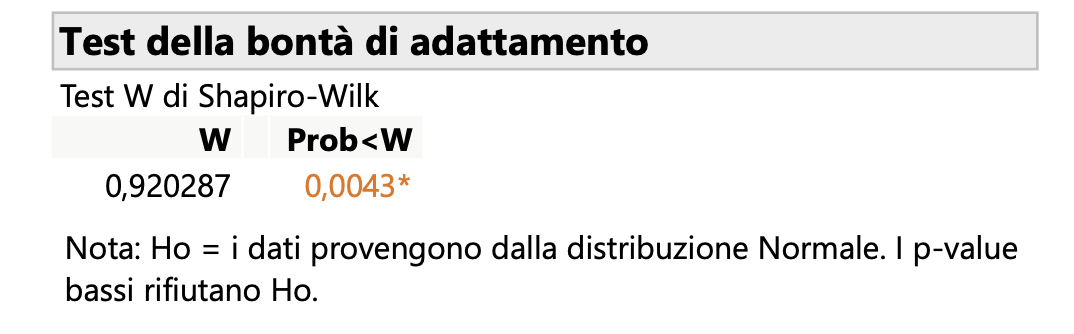
\includegraphics[scale=0.4]{img/chap_1/shwk.png}
    \caption{Test di Shapiro-Wilk}
    \label{fig:shapWilk}
\end{figure}
\noindent
Come si può osservare dalla fidura \ref{fig:qq_res_plot} i residui non sono normali, ipotesi confermata anche da test di Shapiro-Wilk della figura \ref{fig:shapWilk}.\\
Data la non normalità dei campioni si deve procedere per test non parametrici come quello di Kruskal-Wallis, di seguito riportiamo i risultati.\\
\begin{figure}[H]
    \centering
    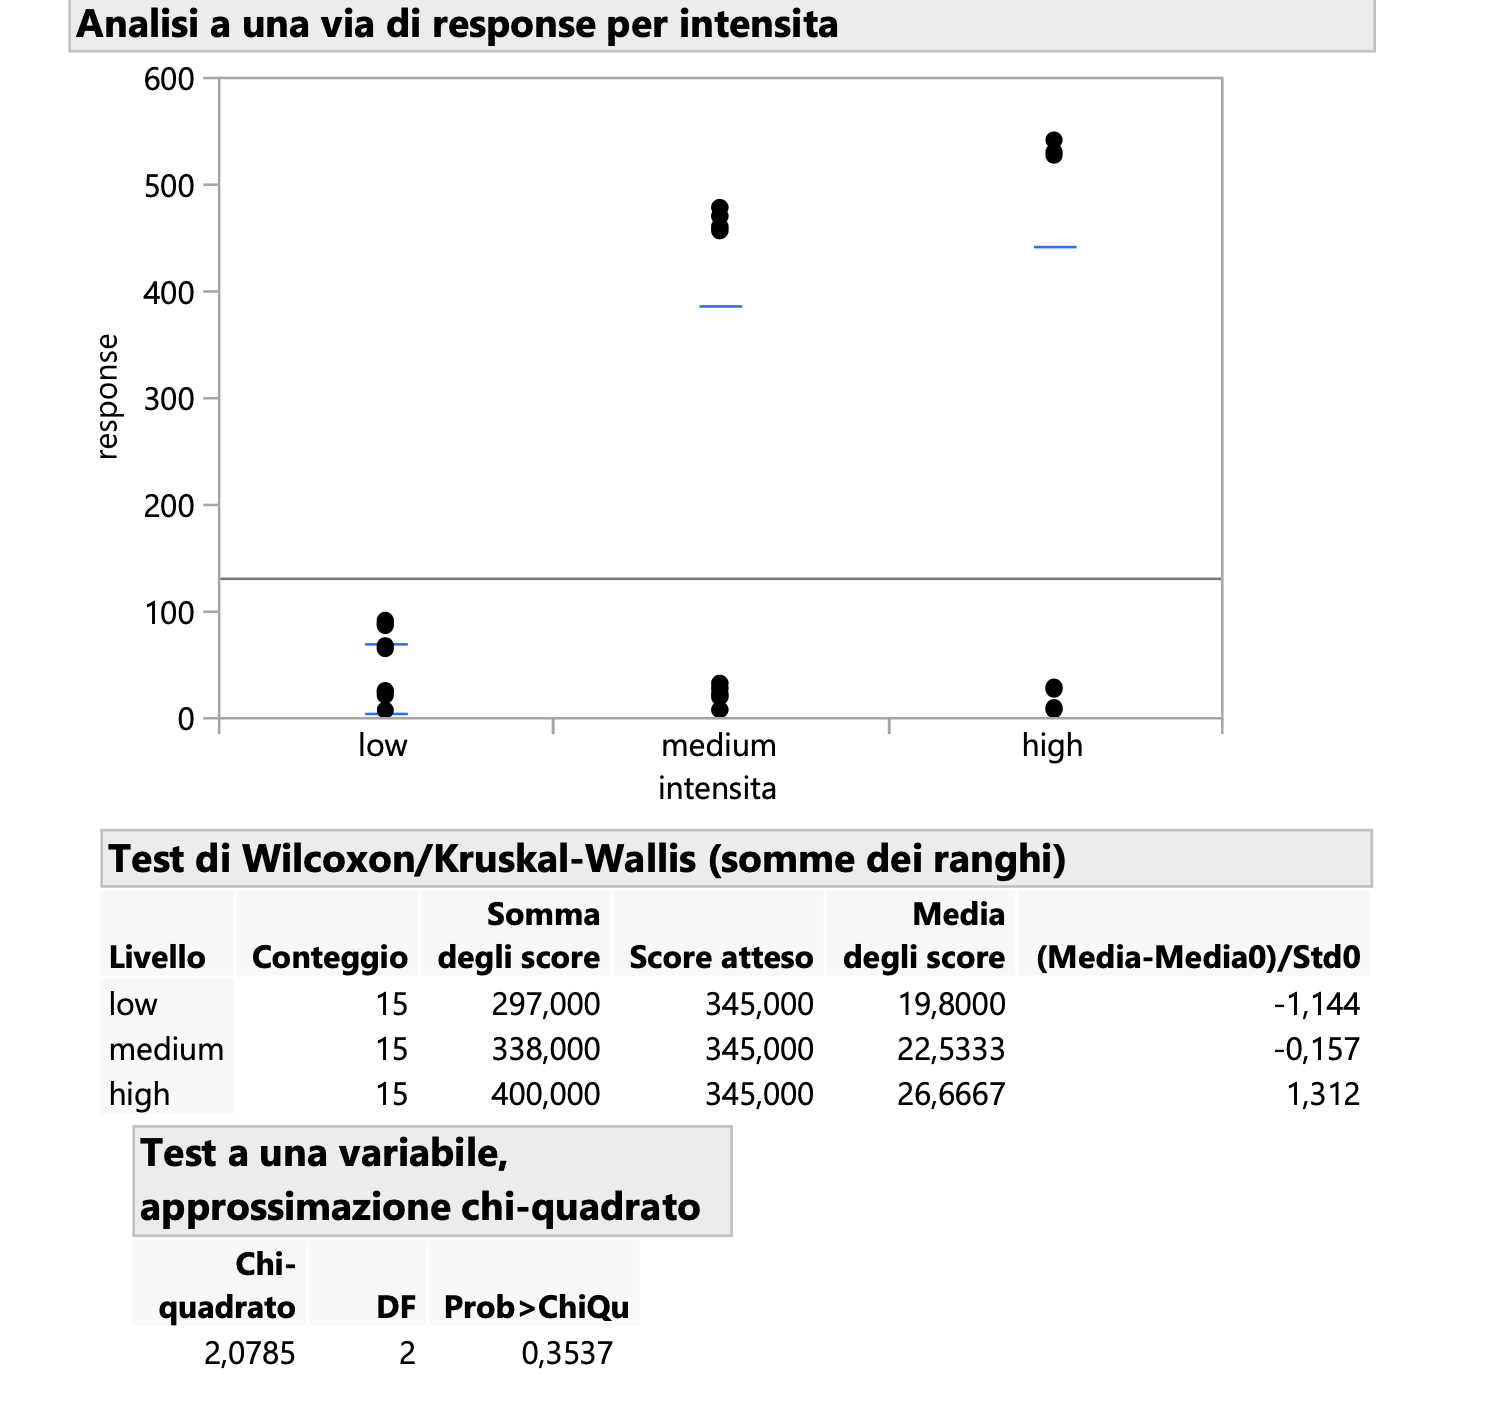
\includegraphics[scale=0.4]{img/chap_1/k_w_intensit.png}
    \caption{Kruskal-Wallis per l'intensità}
    \label{fig:k_w_int}
\end{figure}
\begin{figure}[H]
    \centering
    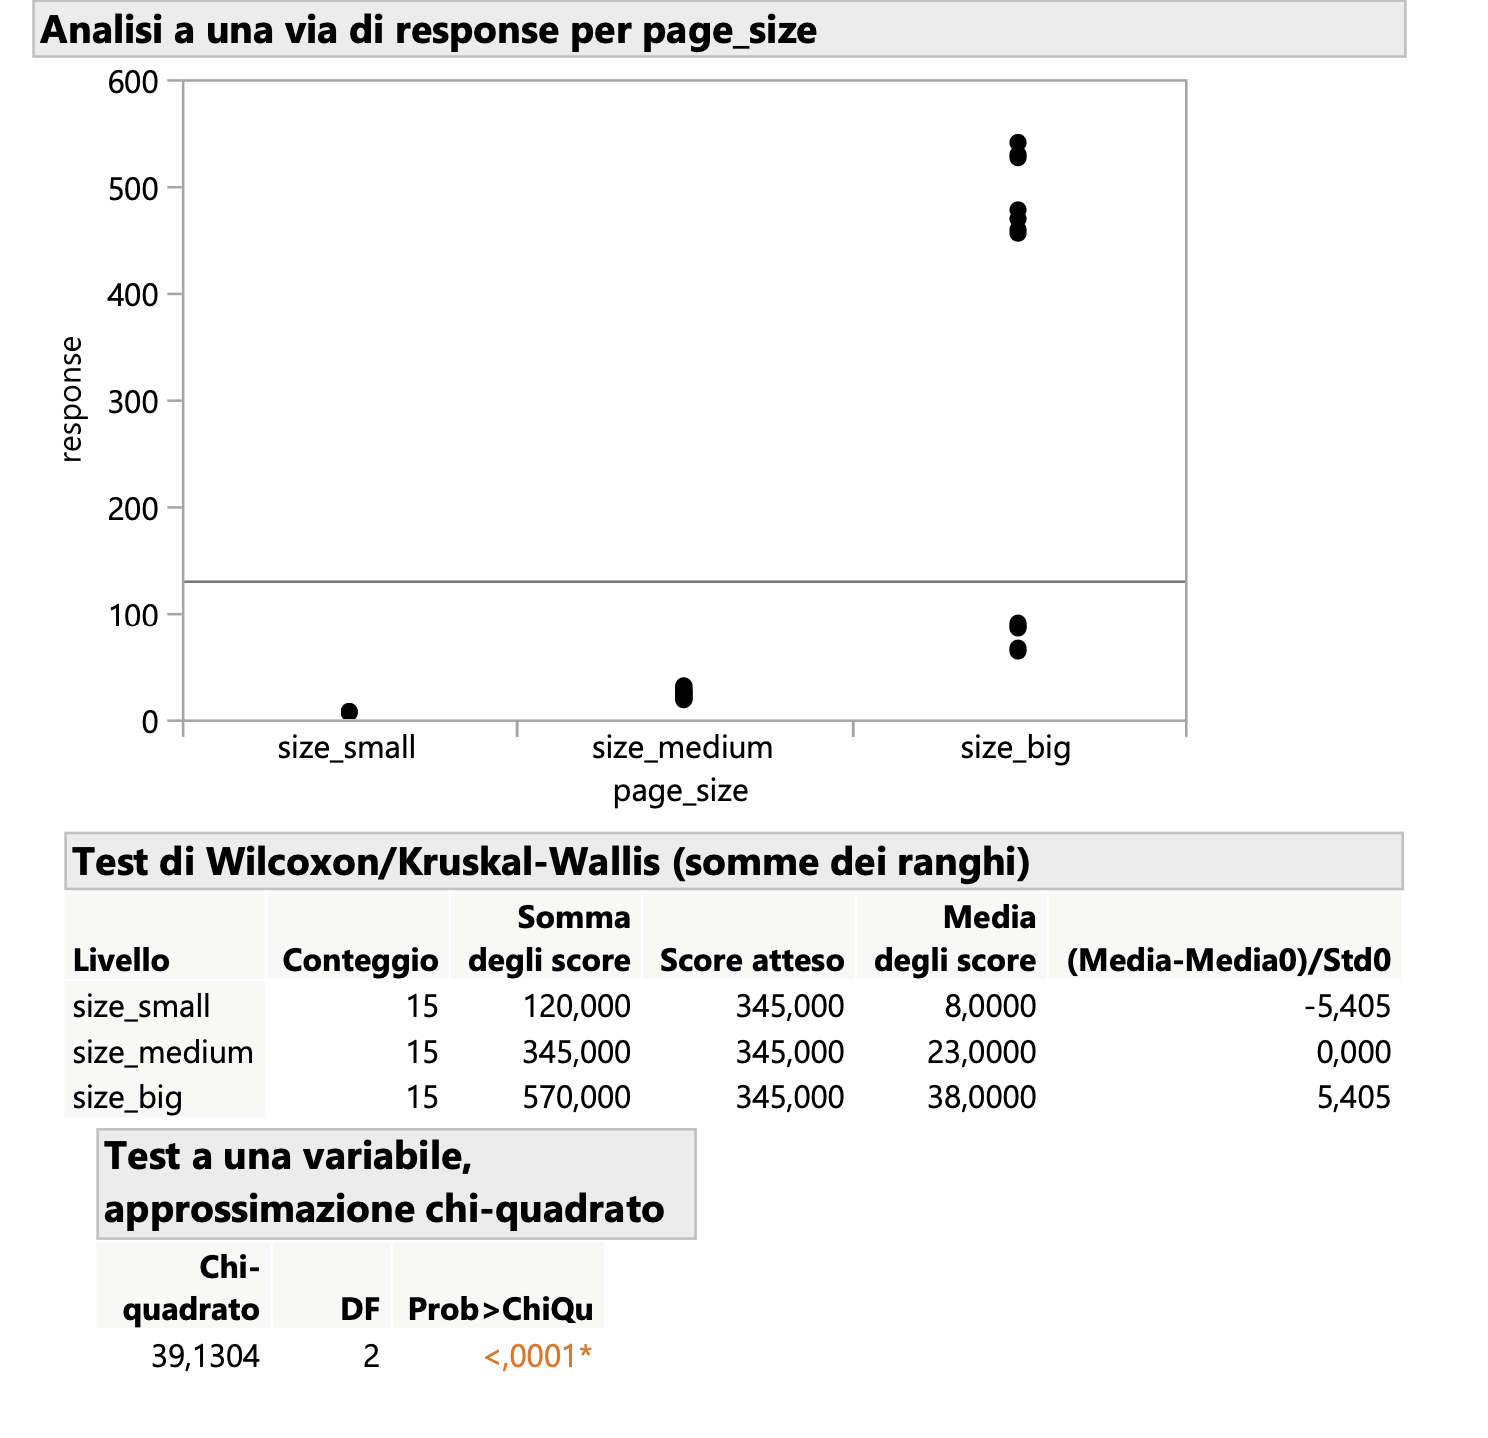
\includegraphics[scale=0.4]{img/chap_1/k_w_pageSize.png}
    \caption{Kruskal-Wallis per page\_size}
    \label{fig:k_w_ps}
\end{figure}
\noindent
Come si può notare dalla figura \ref{fig:k_w_int} il valore di ChiQuadro è molto alto non riuscendo a rigettare l'ipotesi nulla, riportando una non significatività del fattore, diverso invece è per \textit{page\_size} che dalle analisi che è possibile osservare dalla figura \ref{fig:k_w_ps} risulta essere significativo.\\
Dunque in definitiva avremo che \textit{page\_size} è un fattore importante e significativo mentre l'\textit{intensità} non è significativa ed è poco importante.\\ 


  
\chapter{PCA \& Clustering}
In questo capitolo dell'elaborato effettueremo delle analisi di un workload utilizzando tecniche di analisi dati, ovvero PCA e clustering.
In breve la PCA è una procedura statistica che ci permette di riassumere l'informazione contenuta in una grande tabella attraverso un insieme ristretto di indici sintetici facilmente visualizzabili.
Invece il clustering ci permette di dividere dati non etichettati in insiemi differenti detti clusters attraverso una funzione di distanza.
\section{Traccia}
Dato un Workload reale, trovarne uno sintetico rispettando i seguenti requisiti: 

\begin{itemize}
    \item Trovare il miglior trade-off tra numero di componenti principali e numero di cluster
    \item Effettuare una analisi di sensitività, osservando come la varianza cambia al variare di componenti principali e numero di cluster
\end{itemize}
\section{Filtering}
Il primo passo effettuato è stato analizzare i dati grezzi su JMP per capire se si poteva effettuare un filtraggio.\\
Questa analisi hs rivelato, come indica la figura \ref{fig:analisi_filtering} la presenza di colonne a varianza nulla.
\begin{figure}[H]
    \centering
    \includegraphics[scale=0.6]{img/chap_2/PCA_CLUSTERING_1.PNG}
    \caption{Analisi colonne}
    \label{fig:analisi_filtering}
\end{figure}
\noindent
Per tale ragione, non essendo queste colonne portatrici di informazione, sono state eliminate dall'analisi.\\
\textbf{Osservazione:} Quando si parla di eliminare una colonna si intende l'intenzione di non considerarle all'interno dell'analisi ma in fase di selezione del workoad queste ultime devono essere incluse.
Dopo aver fatto una analisi sulle colonne, è stata eseguita una analisi anche riguardante le righe. 
Attraverso l'istogramma frequentista della figura \ref{fig:AnalisiRighe1} sono stati rilevati i seguenti outlier:
\begin{itemize}
    \item \textbf{Riga 1}: con riferimento alla figura \ref{fig:AnalisiRighe1} outlier corrispondente a tutte le grandezze indicate, probabilmente legato ad una condizione di basso carico
    \item \textbf{Righe 2-87}: con riferimento alla figura \ref{fig:AnalisiRighe2} outliers relativi ad una serie di parametri come la memoria (Mem-Free e Writeback). Tali outliers sono legati probabilmente ad una fase transitoria del sistema come l'accensione.
\end{itemize}
\begin{figure}[H]
    \centering
    \includegraphics[scale=0.4]{img/chap_2/Outlier_PCA.PNG}
    \caption{Istogramma frequentista 1}
    \label{fig:AnalisiRighe1}
\end{figure}
\begin{figure}[H]
    \centering
    \includegraphics[scale=0.5]{img/chap_2/righe_escluse.PNG}
    \caption{Istogramma frequentista 2}
    \label{fig:AnalisiRighe2}
\end{figure}
\noindent
Le righe sopracitate sono state eliminate dall'analisi.\\
Da questa procedura di filtering otteniamo un dataset filtrato sul quale effettuare delle analisi.
\section{PCA}
Come detto nell'introduzione, la PCA è una tecnica che effettua una trasformazione generando quelle che si chiamano componenti principali che sono in numero pari alle componenti sulle quali abbiamo effettuato la trasfomazione.\\
Poichè la PCA tiene conto della varianza ci permette di selezionare alcune di queste componenti per ridurre la dimensionalità.\\
Tale analisi viene svolta tramite l'uso di JMP e fornisce i seguenti output: 
\begin{itemize}
    \item \textbf{Loading Plot:} Mostra una matrice  di rappresentazione bidimensionale dei fattori di carico. Tale grafico ci permette di osservare che se due variabili sono simili, sono rappresentate molto vicine tra loro.
    \item \textbf{Score Plot:} mostra una matrice di dispersione per coppie di componenti principali, dunque spiega come si distribuiscono gli elementi in base alle due componenti selezionate.
    \item \textbf{Diagramma a barre:} mostra la varianza conservata da ogni componente principale.
\end{itemize}
Di seguito riportiamo tali plot:\\
\begin{figure}[H]
    \centering
    \includegraphics[scale=0.6]{img/chap_2/PCA_CLUSTERING_2.PNG}
    \caption{output PCA}
    \label{fig:Plot_PCA}
\end{figure}
\noindent
Analizzando più da vicino gli autovalori avremo la seguente situazione:
\begin{figure}[H]
    \centering
    \includegraphics[scale=0.6]{img/chap_2/Osservazione_PCA_Clustering.PNG}
    \caption{Autovalori con varianza}
    \label{fig:Osservazione}
\end{figure}
\noindent
Possiamo notare che gli autovalori dal 18 al 20 può sembrare non spieghino varianza, in realtà aumentando i decimali relativi alla percentuale cumulativa possiamo renderci conto che spiegano varianza, ma è molto piccola.\\
Tale osservazione è visibile nella figura \ref{fig:Osservazione}
Da questa figura ci rendiamo conto che solo il 20 difatto non spiega varianza.
Inoltre abbiamo fatto PCA su 21 dimensioni ma ci ritroviamo solo 20 autovalori.\\
Questo è dovuto ad una correlazione tra \textbf{MemFree} e \textbf{WriteBack}, tale correlazione è evidenziata dalla matrice di correlazione di figura \ref{fig:MatriceDiOsservazione}
\begin{figure}[H]
    \centering
    \includegraphics[scale=0.4]{img/chap_2/PCA_CLUSTERING_4.PNG}
    \caption{Matrice di correlazione}
    \label{fig:MatriceDiOsservazione}
\end{figure}
\section{Clustering}
Dopo aver effettuato l'estrazione delle componenti principali, il prossimo passo da effettuare è quello dell'operazione di clustering. In particolare, il clustering scelto è quello di tipo gerarchico utilizzando come criterio il Metodo di Ward, in modo tale da formare "cluster" in cui le somiglianze tra gli elementi siamo massime e quindi minimizzare la varianza totale all'interno di ogni cluster.
Oltre a minimizzare questa varianza, si vuole anche andare a massimizzare la varianza intercluster, cioè quella tra elementi appartenenti a cluster differenti.
L'output di questa fase è un dendogramma simile a quello di figura \ref{fig:dendogramma}
\begin{figure}[H]
    \centering
    \includegraphics[scale=0.5]{img/chap_2/PCA_CLUSTERING_5.PNG}
    \caption{output Clustering}
    \label{fig:dendogramma}
\end{figure}
\subsection{PCA \& clustering con 4 componenti}
Andando ad effettuare la clusterizzazione con 4 componenti principali, la quantità di varianza che varia in base al numero di cluster scelti è la seguente:
\begin{itemize}
  \item \textbf{5 Cluster:} Varianza pari a 63.96 \% con una perdita del 17,044\% rispetto alla varianza post PCA di 81.004\%
  \item \textbf{30 Cluster:} Varianza pari a 80.42 \% con una perdita del 0.58\% rispetto alla varianza post PCA di 81.004\%
  \item \textbf{50 Cluster:}Varianza pari a 80.63 \% con una perdita del 0,374\% rispetto alla varianza post PCA di 81.004\%
\end{itemize}
Qui di seguito è presentato il dendrogramma, utile per comprendere quanta varianza si perda o si mantenga al variare del numero di cluster.

%inserire dendogramma

\subsection{PCA \& clustering con 5 componenti}
Andando ad effettuare la clusterizzazione con 5 componenti principali, la quantità di varianza che varia in base al numero di cluster scelti è la seguente:
\begin{itemize}
  \item \textbf{5 Cluster:} Varianza pari a 59.02 \% con una perdita del 26,753\% rispetto alla varianza post PCA di 85.773\%
  \item \textbf{30 Cluster:} Varianza pari a 84.92 \% con una perdita del 0,853\% rispetto alla varianza post PCA di 85.773\%
  \item \textbf{50 Cluster:}Varianza pari a 85.32 \% con una perdita del 0,453\% rispetto alla varianza post PCA di 85.773\%
\end{itemize}
Qui di seguito è presentato il dendrogramma, utile per comprendere quanta varianza si perda o si mantenga al variare del numero di cluster.

\subsection{PCA \& clustering con 6 componenti}
Andando ad effettuare la clusterizzazione con 6 componenti principali, la quantità di varianza che varia in base al numero di cluster scelti è la seguente:
\begin{itemize}
  \item \textbf{5 Cluster:} Varianza pari a 56.66 \% con una perdita del 33,21\% rispetto alla varianza post PCA di 89.870\%
  \item \textbf{30 Cluster:} Varianza pari a 87.45 \% con una perdita del 2,42\% rispetto alla varianza post PCA di 89.870\%
  
  \item \textbf{50 Cluster:}Varianza pari a 88.38 \% con una perdita del 1,49\% rispetto alla varianza post PCA di 89.870\%

\end{itemize}
Qui di seguito è presentato il dendrogramma, utile per comprendere quanta varianza si perda o si mantenga al variare del numero di cluster.

\section{Conclusioni}
Analizzando i valori del precedente paragrafo sintetizzati nei seguenti grafici \ref{fig:varianzaSpiegata} e \ref{fig:varianzaPersa}.
Da questi possiamo decidere di selezionare 5 componenti principali e 30 cluster spiegando quindi l'84.92\% di varianza
\begin{figure}[H]
    \centering
    \includegraphics[scale=0.5]{img/chap_2/Varianza.jpeg}
    \caption{Varianza spiegata}
    \label{fig:varianzaSpiegata}
\end{figure}

\begin{figure}[H]
    \centering
    \includegraphics[scale=0.5]{img/chap_2/Loss.jpeg}
    \caption{Varianza persa}
    \label{fig:varianzaPersa}
\end{figure}
\section{Workload sintetico}
Tramite l'analisi effettuata è stato possibile realizzare il workload sintetico seguendo le conclusioni di cui sopra. Da 24 colonne e 3000 righe possiamo disporre di un workload di 24 colonne e solamente 30 righe.
Tale workload è mostrato nella figura \ref{fig:workload}
\begin{figure}[H]
    \centering
    \includegraphics[scale=0.4]{img/chap_2/Workload.png}
    \caption{Workload sintetico}
    \label{fig:workload}
\end{figure}
\chapter{Benchmark}
Usando il benchmark Nbody, il quale simula l'evoluzione di un sistema di N corpi, sotto l'influenza della forza gravitazionale eseguire analisi riguardo due sistemi.
Il benchmark sopra citato stressa:
\begin{itemize}
    \item Sottosistma floating point
    \item Chiamate ricorsive, e quindi stack
\end{itemize}
Le analisi verranno effettuate su due sistemi con lo stesso OS ma con differenti processori.
\section{Attività di Benchmarking}
\begin{center}
    \textit{ A benchmark is the act of running a computer program, a set of programs, or other operations, in order to assess the relative performance of an object, normally by running a number of standard tests and trials against it}
\end{center}
In riferimento alla definizione di \textbf{Fleming, Philip J.; Wallace, John J} nell'articolo \textbf{How not to lie with statistics: the correct way to summarize benchmark results} il benchmark ci permette di confrontare due sistemi riguardo delle loro particolari componenti.\\
Nel nostro caso il benchmark scelto permette di confrontare \textbf{FPU} e \textbf{stack}.
\section{Analisi}
L'obiettivo è dimostrare che i processori delle due macchine non provengono dalla stessa distribuzione poichè pure se appartenenti entrambe alla casa AMD un processore è \textit{desktop} e l'altro è \textit{laptop}.\\
Il sistema operativo è il medesimo.\\
Andremo dunque a definire le seguenti cose:
\begin{itemize}
    \item \textbf{Servizi:} esecuzione di calcoli matematici 
    \item \textbf{Metrica:} tempo (in microsecondi) impiegato per terminare la simulazione
    \item \textbf{Fattori:} Carico CPU, carico memoria ed eventuali attività da parte di altri componenti del sistema.
    \item \textbf{Workload:} Numero di corpi utilizzati nella simulazione
\end{itemize}
Nel seguito sono riportate le specifiche dei due sistemi:
\textbf{Sistema 1:}
\begin{itemize}
    \item \textbf{Processore: } AMD Ryzen 5 3500U
        \begin{itemize}
            \item Frequenza: 2.1GHz
            \item Core: 4
            \item Threads: 8
            \item Cache: 4MB
        \end{itemize}
    \item \textbf{Memoria RAM: } 8 GB 1600 Mhz ddr4
    \item \textbf{SO:} Windows 11 pro 
\end{itemize}

\textbf{Sistema 2:}
\begin{itemize}
    \item \textbf{Processore: } AMD Ryzen 5 2600x
        \begin{itemize}
            \item Frequenza: 3.6GHz
            \item Core: 6
            \item Threads: 12
            \item Cache: 16MB
        \end{itemize}
    \item \textbf{Memoria RAM: } 16 GB 1600 Mhz ddr4
    \item \textbf{SO:} Windows 11 pro 
\end{itemize}
\section{Prelievo dei campioni}
Per il prelievo dei campioni si è seguito un processo che permettesse di raccogliere campioni indipendenti.\\
Per fare ciò si è proceduto a spegnere ed accendere la macchina per svuotare strutture di memoria come RAM e cache.\\
Tale operazione è stata eseguita 30 volte attraverso il seguente comando:
\begin{center}
    \textit{./launch\_nbody.bat -r 4 -n*}
\end{center}
\textbf{r} indica il numero di ripetizioni che sono state fissate a 4 , dunque sono state raccolte 30 osservazioni indipendenti da 4 campioni ciascuna.\\
Questo procedimento è stato effettuato per permettere poi di effettuare un test visivo attraverso un \textbf{qq-plot} della gaussianità della distribuzione dei campioni.\\
\textbf{OSS: }Le osservazioni sono state raccolte in maniera indipendente ma verrà comunque dimostrata l'indipendenza attraverso i diagrammi.\\
\subsection{Calcolo della sample size}
Per capire se i campioni che sono stati prelevati sono sufficienti dobbiamo calcolare quella che è la \textbf{sample size} che ci indica se è possibile approssimare media e varianza del campione con la popolazione, tale calcolo lo effettuiamo per entrambi gli esperimenti.\\
Abbiamo scelto un valore di errore rispetto alla media campionaria dello 1\% ed un intervallo di confidenza del 95\% per cui la nostra sample size è:\\
\begin{center}
    
        $n = (\frac{z_{\frac{\alpha}{2}} \sigma}{E})^2$ \\
        $n_{1\_1} = (\frac{1.96*285}{40})^2 = 7$ \\
        $n_{2\_1} = (\frac{1.96*139}{36})^2 = 2$ \\
        $n_{1\_2} = (\frac{1.96*431}{140})^2 = 2$ \\
        $n_{2\_2} = (\frac{1.96*2036}{156})^2 = 22$ \\
    
\end{center}
Dal calcolo della sample size possiamo considerare il numero dei nostri campioni sufficienti per effettuare l'analisi.\\
\section{Analisi dei dati}
Per effettuare l'analisi delle prestazioni e confrontare i sistemi è stato usato il tool JMP.\\
L'analisi effettuata è di tipo \textbf{paired} in quanto il numero di campioni per ogni osservazioni è lo stesso ed è la stessa anche la corrispondenza degli indici.\\
Per dimostrare l'ipotesi che le osservazioni provengono da popolazioni diverse abbiamo due approcci:

\begin{itemize}
    \item \textbf{T-test(parametrico)}: applicabile se e solo se le due medie campionarie sono approssimativamente distribuite come una normale, ed essendo nel caso two-sample dobbiamo verificare anche l'uguale varianza.
    \item \textbf{Test di Wilcoxon(non parametrico)}: non è richiesta la precedente ipotesi di normalità.Si analizzano le distribuzioni delle differenze campionarie al variare del tipo di sistema e fissando le dimensioni del workload.
\end{itemize}
Sono state effettuate due tipi di osservazioni, una con 25000 corpi e una con 10000 corpi per verificare i due sistemi con due carichi diversi.\\
\subsection{Analisi a 25000}
Di seguito sono presentati i due dataset e le analisi effettuate su di essi.\\
\begin{figure}[H]
    \centering
    \includegraphics[width=.25\textwidth]{img/chap_3/Mariano_25K.png}
    \includegraphics[width=.25\textwidth]{img/chap_3/Frank_25K.png}
    \caption{Dati}
    \label{fig:data}
\end{figure}

\begin{figure}[H]
    \centering
    \includegraphics[scale=0.4]{img/chap_3/25k_mariano.png}
    \caption{25000 corpi Sistema1}
    \label{fig:sis_1_25_k}
\end{figure}

\begin{figure}[H]
    \centering
    \includegraphics[scale=0.4]{img/chap_3/25k_francesco.png}
    \caption{25000 corpi Sistema2}
    \label{fig:sis_2_25_k}
\end{figure}
\noindent
Da una analisi visiva si può evincere che le osservazioni non eccedono le bande di confidenza e questo indicherebbe che queste ultime possono essere considerate derivanti da una distribuzione normale.\\
Abbiamo provveduto al calcolo degli intervalli di confidenza delle due distribuzioni che sono riportati di seguito:\\
\begin{figure}[H]
    \centering
    \includegraphics[width=.45\textwidth]{img/chap_3/f2.png}
    \includegraphics[width=.45\textwidth]{img/chap_3/m2.png}
    \caption{Intervalli di confidenza sistema1(sx) sistema2(dx)}
    \label{fig:sis_2_25_k}
\end{figure}
\noindent
Come si può notare i due intervalli di confidenza non si sovrappongono indicando che i due sistemi sono statisticamente diversi.\\
Per evincere ancora di più questa differenza è stato fatto un test sulle differenze(\textit{zero-mean test}):
\begin{figure}[H]
    \centering
    \includegraphics[scale=0.7]{img/chap_3/dif2.png}
    \caption{zero-mean test 25K}
    \label{fig:zero-mean}
\end{figure}
\noindent
Come si può vedere l'intervallo di confidenza \ref{fig:zero-mean} non contiene lo zero avvalorando la tesi.
\newpage
\subsection{Analisi per 100000 corpi}
Anche in questa sezione sono presentati i dati e le analisi effettuate su di essi.
\begin{figure}[H]
    \centering
    \includegraphics[width=.1\textwidth]{img/chap_3/Mariano_100K.png}
    \includegraphics[width=.1\textwidth]{img/chap_3/Frank_100K.png}
    \caption{Dati}
    \label{fig:data_2}
\end{figure}
\begin{figure}[H]
    \centering
    \includegraphics[scale=0.4]{img/chap_3/100k_mariano.png}
    \caption{100000 corpi Sistema1}
    \label{fig:sis_1_100_k}
\end{figure}

\begin{figure}[H]
    \centering
    \includegraphics[scale=0.4]{img/chap_3/100k_francesco.png}
    \caption{100000 corpi Sistema2}
    \label{fig:sis_2_100_k}
\end{figure}
\noindent
Anche da queste analisi si può notare che le due distribuzioni possono essere assimilate come provenieneti da una distribuzione normale.\\
Anche qui si è effettuato il calcolo degli intervalli di confidenza che sono i seguenti:\\
\begin{figure}[H]
    \centering
    \includegraphics[width=.25\textwidth]{img/chap_3/f4.png}
    \includegraphics[width=.25\textwidth]{img/chap_3/m4.png}
    \caption{Intervalli di confidenza sistema1(sx) sistema2(dx)}
    \label{fig:sis_2_25_k}
\end{figure}
\noindent
Anche in questo caso i due intervalli di confidenza non si sovrappongono avvalorando il fatto che i due sistemi sono statisticamente diversi.\\
Anche in questo caso è stato effettuato uno zero-mean test per avvalorare la tesi:
\begin{figure}[H]
    \centering
    \includegraphics[scale=0.7]{img/chap_3/dif4.png}
    \caption{zero-mean test 100K}
    \label{fig:z_m2}
\end{figure}
\noindent
Anche in questo caso, osservando l'intervallo di confidenza \ref{fig:z_m2} quest'ultimo non contiene lo zero avvalorando il fatto che i due sistemi sono diversi.
\section{Conclusioni}
I test effettuati sono settati su intervalli di confidenza del 95\% dunque siamo al 95\% sicuri che i due sistemi non siano equivalenti statisticamente.\\
In particolare il sistema 1 ha una media più alta del sistema due sia nel caso di 25000 corpi che nel caso dei 100000 corpi, questo indicherebbe il fatto che il sistema 1 statisticamente esegue più lentamente del sistema 2.

\chapter{Regressione}
Un modello regressivo permette di studiare una variabile come funzione di altre variabili.\\
Abbiamo dunque:
\begin{itemize}
    \item \textbf{Variabile di risposta: } variabile stimata
    \item \textbf{Variabili di predizione:} variabili usate per predire la risposta
\end{itemize}
Il modello regressivo lineare semplice assume la seguente forma:
\begin{center}
    $
        Y = aX+b+Z
    $
\end{center}
Z è una v.a che rappresenta l’errore sperimentale.\\
L’obiettivo di questo homework è rilevare e stimare eventuali trend nelle variabili analizzate attraverso modelli regressivi lineari semplici, parametrici e non parametrici.
\section{Mail server 1}
Per il seguente esercizio, è stato applicato un modello regressivo lineare, per cui la risposta è una funzione lineare del predittore.
Come è possibile notare nelle figure sottostanti, sono state eseguite le stime lineari delle variabili byte rec, byte sent e nmail rispetto alla variabile di predizione observation.
E' possibile osservare nel riepilogo della stima l’R-quadro, ovvero il coefficiente di determinazione, che misura il legame tra la variabilità dei dati e la correttezza
del modello statistico utilizzato.
Con tutte e tre le variabili, è possibile osservare un valore molto basso dell'R-quadro, a dimostrazione del fatto che il modello lineare non è il più adatto per predire i dati
\begin{figure}[H]
    \centering
    \includegraphics[width=.30\textwidth]{img/chap_4/Mail_server_1/ByteSent1.png}
    \includegraphics[width=.30\textwidth]{img/chap_4/Mail_server_1/ByteRec1.png}
    \includegraphics[width=.30\textwidth]{img/chap_4/Mail_server_1/Nmail1.png}
    \caption{grafici ByteSent,ByteRec,Nmail1}
    \label{fig:sis_2_25_k}
\end{figure}
\noindent
Sono state analizzate poi le distribuzioni dei residui di byte
rec, byte sent e nmail e in tutti e 3 i casi son presenti outliers che però sono relativi a dati di basso carico, per cui trascurabili nella nostra analisi.

\begin{figure}[H]
    \centering
    \includegraphics[width=.30\textwidth]{img/chap_4/Mail_server_1/ByteSent2.png}
    \includegraphics[width=.30\textwidth]{img/chap_4/Mail_server_1/ByteRec2.png}
    \includegraphics[width=.30\textwidth]{img/chap_4/Mail_server_1/Nmail2.png}
    \caption{grafici ByteSent,ByteRec,Nmail1}
    \label{fig:sis_2_25_k}
\end{figure}
\noindent
In definitiva tutte e 3 le distribuzioni possono assumersi normali.
Si procede ora alla visualizzazione dell’omoschedasticità dei residui e per fare questo, si analizzano i grafici di dispersione dei residui e si verifica  che non vi siano trend.

\begin{figure}[H]
    \centering
    \includegraphics[width=.35\textwidth]{img/chap_4/Mail_server_1/Nmail5.png}
    \includegraphics[width=.35\textwidth]{img/chap_4/Mail_server_1/ByteSent5.png}
    \includegraphics[width=.35\textwidth]{img/chap_4/Mail_server_1/byteRic5.png}
    \caption{dispersione residui Nmail, byte\_inviati, byte\_rec, }
    \label{fig:residui_omoschedastici1}
\end{figure}
\noindent
Come si può vedere dalle \ref{fig:residui_omoschedastici1} questi ultimi sono omoschedas-
tici dunque posso fare affidamento sul test parametrico classico che
restituisce i seguenti risultati:

\begin{figure}[H]
    \centering
    \includegraphics[width=.35\textwidth]{img/chap_4/Mail_server_1/nmail6.png}
    \includegraphics[width=.35\textwidth]{img/chap_4/Mail_server_1/bytesent6.png}
    \includegraphics[width=.35\textwidth]{img/chap_4/Mail_server_1/byteRec6.png}
    \caption{intervalli di confidenza Nmail, byte\_inviati, byte\_rec, }
    \label{fig:residui_omoschedastici}
\end{figure}
\noindent

Il test non riesce a rigettare l’ipotesi nulla sul coefficiente angolare. Ciò evidenzia l’assenza di un trend significativo

\section{Mail server 2}
Anche per il secondo esercizio, procediamo come in quello precedente.
E' possibile osservare nel riepilogo della stima l’R-quadro, ovvero il coefficiente di determinazione, che misura il legame tra la variabilità dei dati e la correttezza
del modello statistico utilizzato.
Con tutte e tre le variabili, è possibile osservare un valore molto basso dell'R-quadro, a dimostrazione del fatto che il modello lineare non è il più adatto per predire i dati
\begin{figure}[H]
    \centering
    \includegraphics[width=.30\textwidth]{img/chap_4/Mail_server_2/ByteSent1.png}
    \includegraphics[width=.30\textwidth]{img/chap_4/Mail_server_2/ByteRec1.png}
    \includegraphics[width=.30\textwidth]{img/chap_4/Mail_server_2/Nmail1.png}
    \caption{grafici ByteSent,ByteRec,Nmail1}
    \label{fig:sis_2_25_k}
\end{figure}
\noindent
Sono state analizzate poi le distribuzioni dei residui di byte
rec, byte sent e nmail e in tutti e 3 i casi son presenti che, a differenza dello scorso caso, non possono essere assunte come normali.
Di conseguenza, è stato applicato un modello non parametrico.
\begin{figure}[H]
    \centering
    \includegraphics[width=.30\textwidth]{img/chap_4/Mail_server_2/ByteSent2.png}
    \includegraphics[width=.30\textwidth]{img/chap_4/Mail_server_2/ByteRec2.png}
    \includegraphics[width=.30\textwidth]{img/chap_4/Mail_server_2/Nmail2.png}
    \caption{distribuzione residui ByteSent,ByteRec,Nmail1}
    \label{fig:sis_2_25_k}
\end{figure}
\noindent
Come modello regressivo non parametrico è stato scelto il test di Mann-
Kendall, che non richiede che i dati siano normalmente distribuiti o lineari.\\
In breve, l’analisi restituirà come risultato un coefficiente di correlazione $\tau$ che varia tra -1 e 1 e un p-value. Un valore negativo indica che le variabili sono inversamente correlate, ovvero che quando una variabile aumenta, l’altra
diminuisce. I valori positivi indicano invece che quando una variabile aumenta,
aumenta anche l’altra.
Un p-value inferiore o uguale a 0,05 avrà come significato che il risultato ottenuto sarà
statisticamente significativo per l’analisi e che l’ipotesi nulla H0, che afferma
che non è presente un trend monotono nella distribuzione, è rifiutata.
Sono riportati di seguito i 3 risultato per i test effettuati.

\begin{table}[htbp]
    \centering
    \label{tab:esempio}
    \begin{tabular}{|c|c|c|c|} % specifica il numero e l'allineamento delle colonne (c = centrato, l = sinistra, r = destra)
        \hline
        Variabile & Variabile by & $\tau$ di Kendall &Prob > |$\tau$| \\ % separa le celle con '&', e termina ogni riga con '\\'
        \hline
        Time & ByteRec & -0.0316 & <0,0012\\
        Time & ByteSent & -0.392 & <0,0001\\
        Time & Nmail & -0.0242 & <0,0138\\
        \hline
    \end{tabular}
\end{table}
\noindent
Dai dati raccolti risulta che, considerato il tasso di significatività standard
pari a $\alpha$ = 0.05, nessuna variabile presenta un trend significativo.

\begin{figure}[H]
    \centering
    \includegraphics[width=.30\textwidth]{img/chap_4/Mail_server_2/ByteSent3.png}
    \includegraphics[width=.30\textwidth]{img/chap_4/Mail_server_2/byteRec3.png}
    \includegraphics[width=.30\textwidth]{img/chap_4/Mail_server_2/Nmail3.png}
    \caption{Test Kendall ByteSent,ByteRec,Nmail1}
    \label{fig:sis_2_25_k}
\end{figure}
\noindent

\section{VMStat}
L’obiettivo è rilevare e stimare eventuali trend sulle 5 variabili utilizzando modelli regressivi lineari semplici, parametrici e/o non parametrici per i tre dataset os1, os2 e os3.
Il significato dei parametri è il seguente:
\begin{itemize}
    \item \textbf{VmSize: }rappresenta l’uso della memoria virtuale dell’intero processo.
    \item \textbf{VmData: }rappresenta la dimensione del segmento di dati del processo;
    \item \textbf{Resident Set Size(RSS): }rappresenta la quantità di memoria fisica attualmente in uso dal processo.Il valore è rappresentato kB.
\end{itemize}
\subsection{VMStat-os1}
Di seguito sono riportati i grafici delle analisi dei modelli lineari applicati ai dati.
\begin{figure}[H]
    \centering
    \includegraphics[width=.35\textwidth]{img/chap_4/Os1/lin_VmSize.png}
    \includegraphics[width=.35\textwidth]{img/chap_4/Os1/lin_VmData.png}
    \caption{grafici VmSize e VmData}
    \label{fig:sis_2_25_k}
\end{figure}
\noindent
Questi due grafici sono relativi ai parametri VmSize e VmData ed avendo loro una funzione costante a tratti non possono essere trattati con modelli lineari semplici.\\
La rilevazione dei trend in questo caso deve procedere per test non parametrici come il \textbf{Mann-Kendall}.\\
\begin{figure}[H]
    \centering
    \includegraphics[width=.25\textwidth]{img/chap_4/Os1/lin_byteletti_1.png}
    \includegraphics[width=.25\textwidth]{img/chap_4/Os1/lin_byteLetti.png}
    \includegraphics[width=.25\textwidth]{img/chap_4/Os1/lin_RSS.png}
    \caption{grafici RSS,Byte letti,byte letti01}
    \label{fig:sis_2_25_k}
\end{figure}
\noindent
Questi grafici suggeriscono che possiamo usare un modello lineare semplice, negli ultimi due casi però il modello non porta con se una grande percentuale di varianza come denunciato dal valore $R^2$ ed $R^2$ corretto.\\
Per capire se possiamo sfruttare un test parametrico analizziamo i residui.
\begin{figure}[H]
    \centering
    \includegraphics[width=.25\textwidth]{img/chap_4/Os1/res_byteletti_1.png}
    \includegraphics[width=.25\textwidth]{img/chap_4/Os1/res_byteletti.png}
    \includegraphics[width=.25\textwidth]{img/chap_4/Os1/res_RSS.png}
    \caption{qq-plot RSS,Byte\_letti,byte\_$letti_{01}$}
    \label{fig:residui}
\end{figure}
\noindent
Gli outlier presenti sono relativi a dati di basso carico per cui trascurabili nella nostra analisi.\\
In definitiva tutte e 3 le distribuzioni possono assumersi normali.\\
Ora devo analizzare l'omoschedasticità dei residui, per fare questo analizzo i grafici di dispersione dei residui e verifico che non vi siano trend.\\
\begin{figure}[H]
    \centering
    \includegraphics[width=.35\textwidth]{img/chap_4/Os1/disp_res_byteletti.png}
    \includegraphics[width=.35\textwidth]{img/chap_4/Os1/disp_res_byteletti_01.png}
    \caption{dispersione residui byte\_letti, byte\_$letti_{01}$}
    \label{fig:residui_omoschedastici}
\end{figure}
\begin{figure}[H]
    \centering
    \includegraphics[scale=0.4]{img/chap_4/Os1/disp_res_rss.png}
    \caption{Dispersione residui RSS}
    \label{fig:residui_non_omoschedastici2}
\end{figure}
\noindent
Come si può vedere dalle figure \ref{fig:residui_omoschedastici2} questi ultimi sono omoschedastici dunque posso fare affidamento sul test parametrico classico che restituisce i seguenti risultati:
\begin{figure}[H]
    \centering
    \includegraphics[width=.35\textwidth]{img/chap_4/Os1/parametri_byteletti.png}
    \includegraphics[width=.35\textwidth]{img/chap_4/Os1/parametri_byteletti_01.png}
    \caption{test parametri byte\_letti, byte\_letti\_01}
    \label{fig:residui_omoschedastici12}
\end{figure}
\noindent
Come si vede i parametri calcolati sono significativi per il parametro \textit{byte\_letti} perchè il test rigetta l'ipotesi nulla (che l'intervallo di confidenza contenga lo 0) per il coefficiente angolare che indica la presenza di un trend significativo, invece per il parametro \textit{byte\_letti01} il test non riesce a rigettare l'ipotesi nulla sul coefficiente angolare che evidenzia l'assenza di un trend significativo.\\
Invece in relazione alla figura \ref{fig:residui_non_omoschedastici12} i residui non sono omoschedastici dunque non possiamo usare un test parametrico come il t-test ma useremo anche qui il test di Mann-Kendall.\\
Di seguito riportiamo i 3 risultati del test di Kendall:
\begin{table}[htbp]
    \centering
    \label{tab:esempio}
    \begin{tabular}{|c|c|c|c|} % specifica il numero e l'allineamento delle colonne (c = centrato, l = sinistra, r = destra)
        \hline
        Variabile & Variabile by & $\tau$ di Kendall &Prob > |$\tau$| \\ % separa le celle con '&', e termina ogni riga con '\\'
        \hline
        Time & VmSize & 0.8076 & <,0001\\
        Time & VmData & 0.8076 & <,0001\\
        Time & RSS & 0.6827 & <,0001\\
        \hline
    \end{tabular}
\end{table}
\\
Quindi la presenza di Trend è presente in tutti i parametri, in particolare il trend presente per RSS suggerisce il fatto che il sistema può raggiungere uno stato di saturazione della memoria poichè tale parametro rappresenta la porzione di memoria ccupata da un processo che è mantenuta nella memoria principale.\\
Attraverso la procedura di Sen è stato possibile calcolare il coefficiente angolare in maniera più precisa restituiendo come coefficiente 0.0049 e come intercetta 42428.80 con una confidenza del 95\% e con il seguente intervallo [0.00488,0.00506].
Stessa cosa si può eseguire per VmSize e VmData avendo per il primo coefficiente 0.0315 e intercetta 738854.39 e intervallo sempre al 95\% pari a [0.0307,0.0323], e per il secondo coefficiente 0.0315 e intercetta 670450.39 e intervallo [0.0307,0.0323].
\subsection{VMStat-os2}
Di seguito sono riportati i grafici delle analisi dei modelli lineari applicati ai dati.
\begin{figure}[H]
    \centering
    \includegraphics[width=.25\textwidth]{img/chap_4/Os2/stim_VMData.png}
    \includegraphics[width=.25\textwidth]{img/chap_4/Os2/stim_VMSize.png}
    \caption{Stima lineare VmData e VmSize}
    \label{fig:residui}
\end{figure}
\noindent
Da questi primi grafici non rileviamo nessuna relazione lineare tra dati dunque per questi parametri verrà effettuato un test non parametrico di tipo Mann-Kendall.
\begin{figure}[H]
    \centering
    \includegraphics[width=.25\textwidth]{img/chap_4/Os2/Stim_Rss.png}
    \includegraphics[width=.25\textwidth]{img/chap_4/Os2/Stim_bytescritti.png}
    \includegraphics[width=.25\textwidth]{img/chap_4/Os2/Stim_byteLetti.png}
    \caption{Stima lineare ByteLetti,Rss e ByteScritti}
    \label{fig:stimaLinBSL}
\end{figure}
\noindent
Facendo riferimento a questi grafici \ref{fig:stimaLinBSL} possiamo rilevare una relazione lineare tra i dati però nel caso di \textit{Byte scritti} e di \textit{Rss}, come rilevabile dal valore di $R^2$ ed $R^2$ corretto il modello non spiega molta varianza.\\
Per tali parametri si procede alla verifica dei residui.
\begin{figure}[H]
    \centering
    \includegraphics[width=.35\textwidth]{img/chap_4/Os2/qq_plot_byteLetti.png}
    \includegraphics[width=.35\textwidth]{img/chap_4/Os2/qq_plot_byteScritti.png}
    \caption{qq-plot residui ByteLetti e ByteScritti}
    \label{fig:qq-plot}
\end{figure}

\begin{figure}[H]
    \centering
    \includegraphics[scale=0.4]{img/chap_4/Os2/qq_plot_nn_rss.png}
    \caption{qq-plot dei residui RSS}
    \label{fig:residui_non_normali}
\end{figure}    
\noindent
Le code iniziali dei residui nei grafici \ref{fig:qq-plot} sono assocuati a dati di basso carico del sistema dunque possono essere non considerati dall'analisi, in definitiva possiamo considerare i residui normali.\\
In riferimento alla figura \ref{fig:residui_non_normali} abbiamo deciso di non considerare la distribuzione dei residui normale e duque per Rss si procederà al test di Mann-Kendall.\\
Per ByteLetti e ByteScritti dobbiamo verificare l'omoschedasticità dei residui.\\
\begin{figure}[H]
    \centering
    \includegraphics[scale=0.4]{img/chap_4/Os2/residui_disp_bletti.png}
    \caption{Dispersione residui Byte letti }
    \label{fig:residui_non_omoschedastici4}
\end{figure}
\noindent
Dalla figura \ref{fig:residui_non_omoschedastici4} si può notare la non omoschedasticità dei residui quindi non possiamo rifarci al classico t-test e dunque bisogna procedere con il test di Mann-Kendall.
\begin{figure}[H]
    \centering
    \includegraphics[scale=0.4]{img/chap_4/Os2/disp_residui_b_scritti.png}
    \caption{Dispersione residui Byte scritti }
    \label{fig:residui_omoschedastici5}
\end{figure}
\noindent
In riferimento alla figura \ref{fig:residui_omoschedastici5} si può notare invece l'omoschedasticità dei residui quindi in questo caso possiamo rifarci al t-test classico, tale test restituisce il seguente risultato:
\begin{figure}[H]
    \centering
    \includegraphics[scale=0.4]{img/chap_4/Os2/test_bscritti.png}
    \caption{Test parametri per byte scritti}
    \label{fig:test_bscritti}
\end{figure}
\noindent
Il test a sinistra di figura \ref{fig:test_bscritti} non rigetta l'ipotesi nulla riguardo la pendenza indicando quindi l'assenza di trend significativi riguardo questo parametro.\\
Di seguito invece sono riportati i risultati dei test non parametrici.
\begin{table}[htbp]
    \centering
    \label{tab:esempio}
    \begin{tabular}{|c|c|c|c|} % specifica il numero e l'allineamento delle colonne (c = centrato, l = sinistra, r = destra)
        \hline
        Variabile & Variabile by & $\tau$ di Kendall &Prob > |$\tau$| \\ % separa le celle con '&', e termina ogni riga con '\\'
        \hline
        Time & VmSize & 0.7065 & <,0001\\
        Time & VmData & 0.7065 & <,0001\\
        Time & RSS & 0.1788 & <,0001\\
        Time & byteLetti & 0.6259 & <,0001\\
        \hline
    \end{tabular}
\end{table} \\
Come si può osservare tutti e quattro i test rigettano l'ipotesi nulla indicandoci la presenza di un trend nei dati.\\
Per avere una stima più precisa del coefficiente si è proceduto ad applicare la procedura si Sen che ha restituito per Rss slope 0.00063 intercetta 42384.85 e intervallo al 95\% pari a [0.001,0.0007], per VmSize e VmData invece per il primo slope 0.00191 intercetta 735790.37 con intervallo [0.0,0.002] e per il secondo slope 0.0019 intercetta 667414.37 e intervallo [0.0,0.002].\\
Invece applicando la procedura di Sen per byteLetti si è ottenuto 114.553 come slope e 77733384.24 intercetta con un intervallo di confidenza la 95\% pari a [112.733 , 116.376] per la slope.
\newpage
\subsection{VMStat-os3}
Di seguito sono riportati i grafici delle analisi dei modelli lineari appli-
cati ai dati.

\begin{figure}[H]
    \centering
    \includegraphics[width=.35\textwidth]{img/chap_4/Os3/VMSize1.png}
    \includegraphics[width=.35\textwidth]{img/chap_4/Os3/VMData1.png}
    \caption{grafici VmSize e VmData}
    \label{fig:sis_2_25_k}
\end{figure}
\noindent
I grafici relativi al VmSize e VmData, avendo una funzione costante a tratti, non possono essere trattati con modelli lineari semplici.
Per rilevare eventuali trend, si utilizzerà il test non parametrico di Mann-Kendall.
\begin{figure}[H]
    \centering
    \includegraphics[width=.25\textwidth]{img/chap_4/Os3/ByteScrittiSec1.png}
    \includegraphics[width=.25\textwidth]{img/chap_4/Os3/ByteLettiSec1.png}
    \includegraphics[width=.25\textwidth]{img/chap_4/Os3/RSS1.png}
    \caption{grafici RSS,Byte letti,byte letti01}
    \label{fig:sis_2_25_k}
\end{figure}
\noindent
Per quanto riguarda questi RSS,ByteSent e ByteLetti, i grafici ci suggeriscono di usare un modello lineare. Per capire se è possibile effettuare un test parametrico, osserviamo i residui.
\begin{figure}[H]
    \centering
    \includegraphics[width=.30\textwidth]{img/chap_4/Os3/ByteScrittiSec2.png}
    \includegraphics[width=.30\textwidth]{img/chap_4/Os3/ByteLettiSec2.png}
    \includegraphics[width=.30\textwidth]{img/chap_4/Os3/RSS2.png}
    \caption{qq-plot RSS,Byte\_letti,byte\_letti01}
    \label{fig:residui}
\end{figure}
\noindent
Gli outlier presenti all'inizio sono relativi a dati di basso carico,però per byte\_scritti e Byte\_Letti 
non si possono considerare lineari.
Si analizza quindi l'omoschedasticità dei residui per RSS
\begin{figure}[H]
    \centering
    \includegraphics[scale=0.4]{img/chap_4/Os3/RSS4.png}
    \caption{Dispersione residui RSS}
    \label{fig:residui_non_omoschedastici}
\end{figure}
\noindent

Come si può notare, i residui non sono omoschedastici
dunque non possiamo usare un test parametrico come il t-test ma useremo anche qui il test di Mann-Kendall.
Di seguito riportiamo i 5 risultati del test di Kendall:
\begin{table}[htbp]
    \centering
    \label{tab:esempio}
    \begin{tabular}{|c|c|c|c|} % specifica il numero e l'allineamento delle colonne (c = centrato, l = sinistra, r = destra)
        \hline
        Variabile & Variabile by & $\tau$ di Kendall &Prob > |$\tau$| \\ % separa le celle con '&', e termina ogni riga con '\\'
        \hline
        Time & VmSize & 0.7832 & <,0001\\
        Time & VmData & 0.7832 & <,0001\\
        Time & letti & -0.0506 & <,0001\\
        Time & scritti & -0.0171 & <,0.0841\\
        Time & RSS & 0.5938 & <,0001\\
        \hline
    \end{tabular}
\end{table}
\\
Quindi la presenza di Trend è presente in tutti i parametri eccetto che per byte letti e scritti. Particolare il trend è presente per RSS suggerisce il fatto che il sistema
può raggiungere uno stato di saturazione della memoria poichè tale parametro rappresenta la porzione di memoria occupata da un processo
che è mantenuta nella memoria principale.
\section{Esercizio Predizioni}
In questa sezione sono presentati 3 dataset i quali tengono traccia della quantità di heap allocata nel tempo e su cui è richiesto effettuare una analisi di tipo failure detection.\\
I passi dunque saranno quelli di identificare un trend nel consumo dell'heap e qualora ci fosse un tren statisticamente significativo stimare il tempo in cui l'heap satura che in questo caso è il superamento della soglia di 1Gb.
\textbf{OSS:} i dati in allocated heap sono rappresentati in byte
\subsection{VMres1}
Per questo primo dataset è stata effettuata una stima lineare che è possibile osservare nella successiva figura.
\begin{figure}[H]
    \centering
    \includegraphics[scale=0.3]{img/chap_4/vmRes1/Stim_lin_VmRes.png}
    \caption{Stima lineare allocated heap}
    \label{fig:stim_lin_VmRes11}
\end{figure}
\noindent
Dalla figura \ref{fig:stim_lin_VmRes11} si può notare che il modello lineare non si adatta bene ai dati, ipotesi che è avvalorata anche dal basso valore di $R^2$ ed $R^2$ corretto.
E' stata effettuata anche una analisi di normalità dei residui
\begin{figure}[H]
    \centering
    \includegraphics[scale=0.4]{img/chap_4/vmRes1/qq_plot_VMres.png}
    \caption{qq-plot residui heap}
    \label{fig:qq_plot_VmRes12}
\end{figure}
Ma da come si può notare dalla figura \ref{fig:qq_plot_VmRes12} questi ultimi non sono normali, dunque si deve procedere a test non parametrico, come Mann-Kendall, per definire se è presente o meno un trend.\\
\begin{table}[htbp]
    \centering
    \label{tab:Mann-kendall4}
    \begin{tabular}{|c|c|c|c|} % specifica il numero e l'allineamento delle colonne (c = centrato, l = sinistra, r = destra)
        \hline
        Variabile & Variabile by & $\tau$ di Kendall &Prob > |$\tau$| \\ % separa le celle con '&', e termina ogni riga con '\\'
        \hline
        Time & Heap & 0.0700 & <,0001\\
        \hline
    \end{tabular}
\end{table}
\\
Come si può vedere dalla tabella \ref{tab:Mann-kendall4} l'ipotesi nulla è rigettata dimostrando la presenza di un trend nei dati, per effettuare la predizione però ci servono le stime di coefficiente ed intercetta.\\
Per le suddette stime si fa uso della procedura di Theil-Sen che ci restituisce la seguente espressione:
\begin{center}
   AllocatedHeap(t) = $0.69t + 6.5*10^6$
   \label{eq:alloc_heap4}
\end{center}
Tale espressione ha come valore di coefficiente angolare una confidenza del 95\% e un intervallo di confidenza pari a [0.564,0.818].\\
Dall'equazione \ref{eq:alloc_heap4} possiamo calcolare il tempo di saturazione risolvendo la sequente equazione(dove l'heap inizia a saturarsi):
\begin{center}
    $
    10^9 = 0.69t+6.5*10^6
    $\\
\end{center}
Da cui 
\begin{center}
    $
    t \approx 45.6$ anni
\end{center}
\newpage
\subsection{VMres2}

Per questo secondo dataset è stata effettuata una stima lineare che è possibile osservare nella successiva figura.
\begin{figure}[H]
    \centering
    \includegraphics[scale=0.3]{img/chap_4/vmRes2/Res1.png}
    \caption{Stima lineare allocated heap}
    \label{fig:stim_lin_VmRes13}
\end{figure}
\noindent
Dalla figura \ref{fig:stim_lin_VmRes13} si può notare che il modello lineare non si adatta bene ai dati, ipotesi che è avvalorata anche dal basso valore di $R^2$ ed $R^2$ corretto.
E' stata effettuata anche una analisi di normalità dei residui
\begin{figure}[H]
    \centering
    \includegraphics[scale=0.4]{img/chap_4/vmRes2/Res2.png}
    \caption{qq-plot residui heap}
    \label{fig:qq_plot_VmRes14}
\end{figure}
Ma da come si può notare dalla figura \ref{fig:qq_plot_VmRes14} questi ultimi non sono normali, dunque si deve procedere a test non parametrico, come Mann-Kendall, per definire se è presente o meno un trend.\\
\begin{table}[htbp]
    \centering
    \begin{tabular}{|c|c|c|c|} % specifica il numero e l'allineamento delle colonne (c = centrato, l = sinistra, r = destra)
        \hline
        Variabile & Variabile by & $\tau$ di Kendall &Prob > |$\tau$| \\ % separa le celle con '&', e termina ogni riga con '\\'
        \hline
        Time & Heap & 0.1378 & <,0001\\
        \hline
    \end{tabular}
\end{table}
\\
Come si può vedere dalla precedente tabella l'ipotesi nulla è rigettata dimostrando la presenza di un trend nei dati, per effettuare la predizione però ci servono le stime di coefficiente ed intercetta.\\
Per le suddette stime si fa uso della procedura di Theil-Sen che ci restituisce la seguente espressione:
\begin{center}
   AllocatedHeap(t) = $0.67t + 5.7*10^6$
   \label{eq:alloc_heap11}
\end{center}
Tale espressione ha come valore di coefficiente angolare una confidenza del 95\% e un intervallo di confidenza pari a [0.605,0.737].\\
Dall'equazione \ref{eq:alloc_heap11} possiamo calcolare il tempo di saturazione risolvendo la sequente equazione(dove l'heap inizia a saturarsi):
\begin{center}
    $
    10^9 = 0.67t+5.7*10^6
    $\\
\end{center}
Da cui 
\begin{center}
    $
    t \approx 47,0$ anni
\end{center}

\subsection{VMres3}
Per questo terzo dataset è stata effettuata una stima lineare che è possibile osservare nella successiva figura.
\begin{figure}[H]
    \centering
    \includegraphics[scale=0.3]{img/chap_4/vmRes3/Res1.png}
    \caption{Stima lineare allocated heap}
    \label{fig:stim_lin_VmRes1}
\end{figure}
\noindent
Dalla figura \ref{fig:stim_lin_VmRes1} si può notare che il modello lineare non si adatta bene ai dati, ipotesi che è avvalorata anche dal basso valore di $R^2$ ed $R^2$ corretto.
E' stata effettuata anche una analisi di normalità dei residui
\begin{figure}[H]
    \centering
    \includegraphics[scale=0.4]{img/chap_4/vmRes3/Res2.png}
    \caption{qq-plot residui heap}
    \label{fig:qq_plot_VmRes1}
\end{figure}
Ma da come si può notare dalla figura \ref{fig:qq_plot_VmRes1} questi ultimi non sono normali, dunque si deve procedere a test non parametrico, come Mann-Kendall, per definire se è presente o meno un trend.\\
\begin{table}[htbp]
    \centering
    \label{tab:Mann-kendall}
    \begin{tabular}{|c|c|c|c|} % specifica il numero e l'allineamento delle colonne (c = centrato, l = sinistra, r = destra)
        \hline
        Variabile & Variabile by & $\tau$ di Kendall &Prob > |$\tau$| \\ % separa le celle con '&', e termina ogni riga con '\\'
        \hline
        Time & Heap & 0.2031 & <,0001\\
        \hline
    \end{tabular}
\end{table}
\\
Come si può vedere dalla tabella \ref{tab:Mann-kendall} l'ipotesi nulla è rigettata dimostrando la presenza di un trend nei dati, per effettuare la predizione però ci servono le stime di coefficiente ed intercetta.\\
Per le suddette stime si fa uso della procedura di Theil-Sen che ci restituisce la seguente espressione:
\begin{center}
   AllocatedHeap(t) = $2.90t + 6.0*10^6$
   \label{eq:alloc_heap}
\end{center}
Tale espressione ha come valore di coefficiente angolare una confidenza del 95\% e un intervallo di confidenza pari a [2.715,3.092].\\
Dall'equazione \ref{eq:alloc_heap} possiamo calcolare il tempo di saturazione risolvendo la sequente equazione(dove l'heap inizia a saturarsi):
\begin{center}
    $
    10^9 = 2.90t+6.0*10^6
    $\\
\end{center}
Da cui 
\begin{center}
    $
    t \approx 10.77$ anni
\end{center}
\chapter{RBD}
RBD sta per \textbf{Reliability Block Diagram} ed è una tecnica per modellare sistemi che sono \textbf{Non-state space}.\\
Tali modelli ci permettono di ottenere una soluzione veloce attraverso l'assunzione che i componenti del sistema siano indipendenti.\\
Dunque vediamo il sistema come una serie di componenti interconnessi tra loro e abbiamo informazioni riguardo:
\begin{itemize}
    \item Probabilità di fallimento
    \item Failure rate
    \item Una distribuzione del tempo al fallimento 
    \item Stady state e istantanea unavailability
\end{itemize}
Le assunzioni di tale tecnica sono:
\begin{itemize}
    \item I failure nei moduli sono indipendenti
    \item Se un modulo fallisce rimarrà nel suo stato di fallimento
    \item Un sistema è fallito se non provvede ad un set minimo di moduli funzionali
\end{itemize}
Di sequito sono risolti degli esercizi riguardanti gli RBD.
\section{Esercizio 1}
\begin{figure}[H]
    \centering
    \includegraphics[scale=0.5]{img/chap_5/Ex1.png}
    \caption{Esercizio 1}
    \label{fig:Ex_1}
\end{figure}
\noindent
In prima analisi notiamo i primi collegamenti parallelo serie(denotiamo con || un parallelo e con - una serie), in particolare abbiamo \textbf{C1||C2} e \textbf{C5-C6}
Da cui avremo:
\begin{center}
    $
        R_{C1||C2} = 1−(1−R)(1R) = 1−(1−R)^2 
        R_{C5-C6} = R^2
    $
\end{center} 
Il nuovo schema sarà:
\begin{figure}[H]
    \centering
    \includegraphics[scale=0.5]{img/chap_5/Ex1_1.png}
    \caption{Schema trasformato}
    \label{fig:Ex_1_1}
\end{figure}
\noindent
Non potendo identificare altre strutture serie o parallelo dobbiamo procedere con il teorema del condizionamento su C4.\\
Per prima cosa possiamo ricavare un upper bound con la tecnica dei success path che sono:
\begin{itemize}
    \item C1||C2 \textminus{} C4
    \item C3 \textminus{} C4
    \item C3 \textminus{} (C5 \textminus{} C6)
\end{itemize}
Otteniamo dunque il seguente Upper-bound:
\begin{center}
    $
        R_{sys} \leq 1-(1-R^2)^3(1-R^3)
    $
\end{center}
Essendoci ricavati un upper bound possiamo procedere con l'analisi attraverso il condizionamento.\\
Per il teorema del condizionamento ho:\\
\begin{center}
    $R_{sys}$ = $R*P$(sistema funziona | C è UP) $+ (1-R) \cdot $P(sistema funziona|C è DOWN)
\end{center}
Di seguito riportiamo i due schemi uno con C4 DOWN e l'altro con C4 UP.\\
\begin{figure}[H]
    \centering
    \includegraphics[scale=0.5]{img/chap_5/Ex_1_2.png}
    \caption{C4 UP}
    \label{fig:Ex_1_2}
\end{figure}
\begin{figure}[H]
    \centering
    \includegraphics[scale=0.5]{img/chap_5/Ex_1_3.png}
    \caption{C4 DOWN}
    \label{fig:Ex_1_3}
\end{figure}
\noindent
Riguardo la figura \ref{fig:Ex_1_3} abbiamo C3-(C5-C6) che danno la seguente reliability:
\begin{center}
 P(sistema funziona | C è UP) =  $R^3$
\end{center}
Invece riguardo la figura \ref{fig:Ex_1_2} si può dimostrare, riapplicando il teorema del condizionamento che abbiamo il seguente risultato:\\
\begin{center}
    P(sistema funziona | C è UP) =  $1-(1-R)^3$
\end{center}
Andando a sostituire nella formula del teorema del condizionamento avrò:\\
\begin{center}
     $R_{sys}$ = $R[1-(1-R)^3] + R^3(1-R)$
\end{center}
Avendo un reliability di tipo esponenziale con failure rate $\lambda$, sostituendo ho:\\
\begin{center}
    $R_{sys}(t) = -2e^{-3\lambda t } + 3e^{-2\lambda t}$
\end{center}
Volendo calcolare l'MTTF avrò:
\begin{center}
    $
        \int_0^{\infty} R_{sys}(t) dt = \frac{5}{6\lambda}
    $
\end{center}
\section{Esercizio 2}

\begin{figure}[H]
    \centering
    \includegraphics[scale=0.5]{img/chap_5/Ex2.png}
    \caption{Esercizio 2}
    \label{fig:Ex_2}
\end{figure}
\noindent
Da una prima analisi qualitativa si può notare che in termini di reliability il secondo sistema è più reliable del primo avendo un numero di \textbf{success path} maggiore.\\
Il primo sistema è composto dal parallelo di \textit{m} catene composte da una serie di \textit{s} sistemi.\\
In termini di reliability avremo per il primo sistema la seguente espressione di reliability:
\begin{center}
    $
        R_{sys1} = [1-(1-R^s)^m]
    $
\end{center}
Il secondo sistema invece è composto da una serie di \textit{s} paralleli di \textit{m} sottosistemi.\\
Avremo dunque la seguente reliability:
\begin{center}
    $
        R_{sys2} = [1-(1-R)^m]^s
    $
\end{center}
Per i valori dell'esercizio avrò:
\begin{center}
    $
    R_{sys1} = [1-(1-R^4)^2] 
    R_{sys2} = [1-(1-R)^2]^4 
    $
\end{center}
Per effettuare la comparazione tra i due sistemi dobbiamo fissare il failure rate $\lambda$ e consideriamo R = $e^{-\lambda t}$.
Il parametro failure rate lo prendiamo dall'MTTF che è stato posto a 800h.
Ricordando che MTTF = $\frac{1}{\lambda}$ nel particolare caso di reliability esponenziale, dunque $\lambda = \frac{1}{800h}$. 
Di seguito riportiamo il plot della reliability in funzione del tempo:

\begin{figure}[H]
    \centering
    \includegraphics[scale=0.5]{img/chap_5/plt_rel.png}
    \caption{plot reliability}
    \label{fig:plt_rel}
\end{figure}
\noindent
Dal grafico \ref{fig:plt_rel} si può notare che il sistema2, a prescindere dal valore del mission time, risulta essere drasticamente più reliable del primo.\\
Se supponiamo un mission time di 350h possiamo notare che il primo sistema ha una reliability di circa il 32\% mentre il secondo di circa il 58\%.
Fissato questo mission time per rendere equivalenti i due sistemi modificando il primo si può lavorare sul numero di catene \textit{m} imponendo la seguente equazione:
\begin{center}
    $
    1-(1-R^4)^m = \frac{58}{100}
    $
\end{center}
Da cui possiamo ottenere: 
+\begin{center}
    $
    m = \lceil \log_{1-\exp^{-\frac{4 \cdot 350}{800}}}(1-\frac{58}{100})\rceil = 5
    $
\end{center}
Si può dimostrare che non si può agire sul parametro \textit{s} per migliorare lo schema.\\
Di seguito si riporta l'andamento grafico che conferma circa l'equivalenza tra i due sistemi per un mission time di 300h. 

\begin{figure}[H]
    \centering
    \includegraphics[scale=0.6]{img/chap_5/plt_rel_2.png}
    \caption{plot confronto}
    \label{fig:plt_rel2}
\end{figure}
\noindent

\section{Esercizio 3}
\begin{figure}[H]
    \centering
    \includegraphics[scale=0.6]{img/chap_5/ex_3.png}
    \caption{Esercizio 3}
    \label{fig:ex_3}
\end{figure}
\noindent
Come riportato dalla traccia, abbiamo una topologia skip-ring la quale è una topologia che ci permette il funzionamento anche in presenza di di fallimenti, in particolare la rete funziona se non falliscono due nodi adiacenti.\\
Il sistema presentato può essere assunto come un sistema M-out-of-N, ovvero sistemi composti da N componenti, ciascuno con una certa reliability R, dei quali almeno M devono funzionare.\\
La formula della reliability per questi sistemi è la seguente:
\begin{center}
    $
    R_{MN} = \sum^{N-M}_{i=0} \binom{N}{i} \cdot R^{N-i} \cdot (1-R)^i
    $
\end{center}
Per studiare questo caso però dobbiamo sottrarre i casi in cui la rete non funziona, e quindi assumere un certo numero di fallimenti ed enumerare le possibili combinazioni che portano al fallimenti di nodi adiacenti.\\
Enumerando i vari casi si può vedere che per un numero di fallimenti i $\geq$ 5 la rete non funziona poichè c'è almeno una coppia di nodi adiacenti che non funziona.\\
Enumerando le varie situazioni abbiamo le seguenti casistiche di reliability:
\begin{itemize}
    \item i = 0 se tutti i nodi funzionano correttamente, il sistema funziona ed avrò dunque:
    \begin{center}
        $
        \binom{8}{0} \cdot R^{8} \cdot (1-R)^0 = R^8
        $
    \end{center}
    \item i=1, se fallisce un solo nodo, il sistema continua a funzionare per la caratteristica della topologia, dunque avrò:
        \begin{center}
        $
        \binom{8}{1} \cdot R^{7} \cdot (1-R)^1 = 8R^7 \cdot (1-R)
        $
        \end{center}
    \item i = 2, in questo caso potremmo avere dei fallimenti se falliscono due nodi adiacenti. Si può vedere che le combinazioni possibili sono 8 enumerandole, allora avrò
        \begin{center}
        $
        (\binom{8}{2}-8) \cdot R^{6} \cdot (1-R)^2 = 20R^6 \cdot (1-R)^2
        $
        \end{center}
       \item i = 3 abbiamo due casi in cui il sistema non funziona
       \begin{itemize}
           \item falliscono 3 nodi adiacenti: 8 combinazioni di non funzionamento
           \item falliscono 2 nodi adiacenti e 1 non adiacente: in tale caso abbiamo che ogni coppia di nodi adiacenti ha 4 nodi non adiacenti che possono fallire, dunque 8*4 combinazioni, ovvero 32 
       \end{itemize}
       Per cui:
        \begin{center}
        $
        (\binom{8}{3}-(8+32)) \cdot R^{5}*(1-R)^3 = 16R^5 \cdot (1-R)^3
        $
        \end{center}
    \item i = 4, in questo caso è utile valutare le condizione di funzionamento che quelle di malfunzionamento, in particolare le condizioni di funzionamento essendo 8 nodi, i nodi falliti devono alternarsi, in tale caso abbiamo solo due combinazioni di funzionamento, dunque:
        \begin{center}
        $
        2 \cdot R^4(1-R)^4
        $
        \end{center}
\end{itemize}
La reliability del sistema è la somma di quelle sopra riportate.
    \[
        \resizebox{1\textwidth}{!}{$
            R_{sys} = R^8+8R^7 \cdot (1-R)+20R^6 \cdot (1-R)^2+16R^5 \cdot (1-R)^3+2 \cdot R^4(1-R)^4
        $}
    \]
Supponendo che la reliability di un singolo componente segua una legge esponenziale con $\lambda = 0.005$ e quindi la reliability di ogni nodo ha R=$e^{- \lambda t}$ posso calcolare la reliability per un mission time di 48 ore che sarà:
\begin{center}
    $
    R_{sys}(48) = 0.73
    $
\end{center}
Di seguito riportiamo anche il grafico della funzione di reliability del sistema
\begin{figure}[H]
    \centering
    \includegraphics[scale=0.6]{img/chap_5/plt_skip.png}
    \caption{Reliability skip-ring}
    \label{fig:plt_skip}
\end{figure}

\section{Esercizio 4}
\begin{figure}[H]
    \centering
    \includegraphics[scale=0.6]{img/chap_5/ex_4.png}
    \caption{Esercizio 4}
    \label{fig:plt_skip}
\end{figure}
\subsection{Confronto 1}
In termini di success path i due sistemi sono uguali (entrambe presentano 2 success path) ma eseguendo una analisi qualitativa se il sistema A fallisce nello schema di destra, l'intero sistema non funziona facendo dunque di A un single point of failure (SPOF).\\
Eseguendo i calcoli avremo:
\begin{center}
    $
    R_{sys1} = 1-(1-R_a \cdot R_b)(R_a \cdot R_c)
    R_{sys2} = R_a \cdot [1-(1-R_b)(1-R_b)]
    $
\end{center}
Ora possiamo particolarizzare per il valore di reliability che ci è stato fornito ricordando che MTTF = $\frac{1}{\lambda}$ e la reliability assume una occorrenza esponenziale, dunque $R=e^{-\lambda t}$.
Avendo fatto le seguenti considerazioni i valori del failure rate saranno:
\begin{itemize}
    \item $\lambda_a = 0.002$
    \item $\lambda_b = 0.00011$
    \item $\lambda_a = 0.0001$
\end{itemize}
Di seguito riportiamo la reliability in funzione del mission time.\\
\begin{figure}[H]
    \centering
    \includegraphics[scale=0.6]{img/chap_5/plt_confr_1.png}
    \caption{confronto tra i due sistemi}
    \label{fig:cofr_sys}
\end{figure}
Come si può vedere dal grafico \ref{fig:cofr_sys} il primo sistema è sempre più reliable del secondo.
\subsection{Confronto 2}
In questo confronto si può notare che il primo ha più success path del secondo e quindi in prima analisi si potrebbe pensare che il primo sia più reliable del secondo.\\
Però possiamo notare una prima cosa, i due sistemi presentano lo stesso SPOF che sarebbe A.\\
Procedendo con una analisi grafica avremo le seguenti espressioni per i due sistemi:
\begin{center}
    $
    R_{sys1} = R_a \cdot [1-(1-R_a)(1-R_b)]
    R_{sys2} = R_a
    $
\end{center}
Di seguito riportiamo il grafico della reliability dei due sistemi:
\begin{figure}[H]
    \centering
    \includegraphics[scale=0.6]{img/chap_5/plt_confr_2.png}
    \caption{confronto tra i due sistemi}
    \label{fig:cofr2_sys}
\end{figure}
\noindent
Come si può vedere dal grafico \ref{fig:cofr2_sys} il secondo sistema è di poco più reliable del primo con i parametri di MTTF forniti.\\
Quindi in termini di costo si potrebbe optare di usare più il sistema a destra rispetto che il sistema a sinistra che sicuramente costa di più.
\subsection{Confronto 3}
In questo caso abbiamo una situazione simile al secondo confronto poichè abbiamo due elementi serie comuni tra i due schemi.\\
Il primo schema ha 2 success path quindi è candidato ad essere più reliable di quello a destra, però ci interessa capire se questa differenza è molto ampia o no.\\
Di seguito riportiamo le espressioni dei due sistemi:
\begin{center}
    $
    R_{sys1} = R_a R_b \cdot [1-(1-R_a)(1-R_b)]
    R_{sys2} = R_a R_b
    $
\end{center}
Di seguito riportiamo il grafico della reliability dei due sistemi:
\begin{figure}[H]
    \centering
    \includegraphics[scale=0.6]{img/chap_5/plt_confr_3.png}
    \caption{confronto tra i due sistemi}
    \label{fig:cofr3_sys}
\end{figure}
\noindent
Anche in questo caso la differenza è poca quindi in termini di costo potrebbe essere più conveniente usare il sistema a destra poichè più economico sicuramente rispetto a quello di sinistra.
\subsection{Confronto 4}
Per quanto riguarda l'ultimo confronto si può vedere che il sistema di sinistra ha più success path di quello a destra e quindi possiano aspettarci una reliability più alta.\\
D'altronde l'osservazione è anche intuitiva poichè il sistema di sinistra introduce ridondanza mentre quello di destra no.\\
Procedendo in modo analitico avremo:
\begin{center}
    $
    R_{sys1} = 1-(1-R_a)(1-R_a R_b)
    R_{sys2} = R_a 
    $ 
\end{center}
Di seguito riportiamo il grafico della reliability dei due sistemi:
\begin{figure}[H]
    \centering
    \includegraphics[scale=0.5]{img/chap_5/plt_confr_4.png}
    \caption{confronto tra i due sistemi}
    \label{fig:cofr4_sys}
\end{figure}
\noindent
Come potevamo aspettarci la reliability del sistema a sinistra è molto migliore rispetto a quello a destra.
\section{Esercizio 5}

\begin{figure}[H]
    \centering
    \includegraphics[scale=0.5]{img/chap_5/ex_5.png}
    \caption{Esercizio 5}
    \label{fig:ex_5}
\end{figure}
\noindent
Del sistema in figura \ref{fig:ex_5} possiamo disegnare quello che è l'RBD caratterizzato dalla serie di tutti i componenti necessari al funzionamento del veivolo ed il parallelo delle repliche.\\
Lo schema risultante sarà quello in figura \ref{fig:rbd_5}
\begin{figure}[H]
    \centering
    \includegraphics[scale=0.5]{img/chap_5/rbd_5.png}
    \caption{RBD elicottero}
    \label{fig:rbd_5}
\end{figure}
\noindent
Di questo RBD possiamo calcolare la reliability complessiva del sistema:
\begin{center}
    $
    R_{sys} = [1-(1-R_p)^2] \cdot [1-(1-R_t)^2] \cdot [1-(1-R_{busA})^2] \cdot [1-(1-R_{busB})^2] \cdot [1-(1-R_{INS})(1-R_D)(1-(1-R_{AHRS})^3]
    $
\end{center}
Per effettuare l'FTA si è usato il tool \textbf{Top Event FTA} andando a modellare il sistema come un \textit{Fault Tree}.\\
Il Fault tree è ottenibile dall'RBD andando a sostituire a tutti i paralleli delle porte OR e a tutte le serie delle porte AND.\\
Facendo così otterremo il seguente schema:
\begin{figure}[H]
    \centering
    \includegraphics[scale=0.5]{img/chap_5/FTA_elicottero.png}
    \caption{FT elicottero}
    \label{fig:ft_elicottero}
\end{figure}
\noindent
Usando l'algoritmo MOCUS per individuare i \textit{Minimal Cut Set}, ovvero insiemi minimali di sottoinsiemi il cui malfunzionamento causa il fallimento del sistema.\\
In particolare quelli individuati sono i seguenti:
\begin{figure}[H]
    \centering
    \includegraphics[scale=0.4]{img/chap_5/minCutSet.png}
    \caption{Minimal Cut Set}
    \label{fig:cutSet}
\end{figure}
\noindent
Ora è richiesto di calcolare la reliability per 1 ora di volo dati i valori di MTTF riportati in tabella e supponendo una distribuzione esponenziale assumendo una coverage iniziale perfetta.\\
Secondo i valori riportati avremo:
\begin{center}
    $
    R_{sys}(t=1h) = 0.9999999400737104
    $
\end{center}
Per tale richiesta è stato anche disegnata la funzione di reliability del sistema.\\
\begin{figure}[H]
    \centering
    \includegraphics[scale=0.4]{img/chap_5/rel_graph.png}
    \caption{reliability elicottero}
    \label{fig:graph_rel}
\end{figure}
\noindent
Come ultima parte si richiede di calcolare la reliability per un ora di volo considerando un fattore di coverage per la \textit{fault detection and reconfiguration} della processing unit.\\
In particolare stiamo assumendo un processore \textit{spare} ovvero di ricambio, modifica la formula della reliability nel seguente modo:
\begin{center}
    $
    R_{sys} = [R_p+c(1-R_p)R_p] \cdot [1-(1-R_t)^2] \cdot [1-(1-R_{busA})^2] \cdot [1-(1-R_{busB})^2] \cdot [1-(1-R_{INS})(1-R_D)(1-(1-R_{AHRS})^3]
    $
\end{center}
Dobbiamo calcolare c tale che $R_{sys} \geq 0.99999$ per 1 ora di volo, risolvendo avremo almeno: 
\begin{center}
    $
        c \simeq 0.91
    $
\end{center}

\chapter{FFDA}
L'obiettivo della Field Failure Data Analysis(FFDA) è quello di ricavare delle misure di \textit{dependability} del sistema reale attraverso azioni di \textit{logging and collection, filtering and manipulation} e analisi di failure che si verificano durante la normale fase operativa del sistema.\\
Questa tecnica measurement based è estremamente affidabile e consente un analisi dettagliata e precisa delle proprietà di un sistema, ma è molto costosa e difficilmente generalizzabile.\\
In questo capitolo si descrive lo svolgimento di una \textbf{log-based FFDA} condotta su due sistemi:
\begin{itemize}
\item \textbf{Mercury}: situato presso il NCSA
\item \textbf{BlueGene}: situato presso LLNL
\end{itemize}
\section{Analisi sistema Mecury}
Il supercalcolatore Mercury è costituito da nodi IBM attraverso una architettura 3-layered + nodo di management.\\
Su ogni nodo è installato un sistema \textbf{RedHat 9.0 OS} e i log sono stati raccolti attraverso \textbf{syslog deamon}.\\
Si hanno a disposizione dei log già filtrati e deperametrizzati tramite whitelisting con dizionario che ammontano ad 80854 di severity \textbf{FATAL}.\\
Ogni entry ha un formato pari a:
\begin{center}
timestamp - nodo - sottosistema originante - descrizione
\end{center}
Riportiamo di seguito le categorie di errore che ritroviamo nei log:
\begin{itemize}
\item \textbf{DEV}:  Platform PCI Component Error Info Section;
\item \textbf{MEM}: MEM: Mem Error Detail: Physical Address *, Address Mask:*, Node:*, Card:*, Module: *, Bank:*, Device:*,Row:*,Column:*
\item \textbf{NET}: Connection down
\item \textbf{I-O}:  error, dev *:* (hda), sector *; hda: packet command error:
\item \textbf{PRO}: BEGIN HARDWARE ERROR STATE AT CMC. 
\end{itemize}
In generale abbiamo 50 messaggi di errore univoci che hanno generato 80854 entry.
\subsection{Analisi di alto livello del sistema}
La prima analisi che si è svolta è una analisi di alto livello riguardo gli errori del sistema, quindi quale è il più frequente come errore e quale nodo ha la più alta frequenza di fault.\\
In particolare si può notare, dalla figura \ref{fig:freqFaultNode} il nodo tg-c401 è quello che ha associato il più alto numero di errori con circa il 77\% di essi associati a questo nodo 
\begin{figure}[H]
    \centering
    \includegraphics[scale=0.4]{img/chap_6/FaultFreqNode.png}
    \caption{Frequenza di faults per nodo}
    \label{fig:freqFaultNode}
\end{figure}
\noindent
Inoltre si è osservato anche, secondo il grafico \ref{fig:freqFauls} che la categoria più frequente è quella DEV con il 71\% di occorrenze.
\begin{figure}[H]
    \centering
    \includegraphics[scale=0.4]{img/chap_6/FaultFreq.png}
    \caption{Frequenza di tipi faults}
    \label{fig:freqFauls}
\end{figure}
\noindent
Analizzando il grafico \ref{fig:freqFaultNode} si è deciso di analizzare il breakup delle entry per nodo e categoria solo per i primi 8 nodi presenti nel grafico.\\
Si può notare dal grafico \ref{fig:freqFaulsTypeNode} che i nodi provenienti dallo stello layer esibiscono simili comportamenti di failure.
\begin{figure}[H]
    \centering
    \includegraphics[scale=0.3]{img/chap_6/FaultTypeNodeFreq.png}
    \caption{Frequenza di tipi faults per nodo}
    \label{fig:freqFaulsTypeNode}
\end{figure}
\noindent
Ad esempio i nodi computazionali tendono ad avere errori di tipo DEV e MEM, mentre i nodi di storage esibiscono errori di tipo I/O.\\
Il nodo \textit{tg-master} è caratterizzato dall'occorrenza NET error probabilmente causati da errori di comunicazione con altri nodi.\\
\subsection{Coalescenze window and content-based coalescence technique}
L'analisi di coalescenza è una fase molto critica nell'analisi dei log poichè ha lo scopo di ricostruire il processo di fallimento del sistema raggruppando gli eventi scaturiti dalla stessa failure.\\
Per effettuare tale analisi dobbiamo determinare una \textit{coalescence window}(cwin) per applicare una coalescenza temporale (\textbf{toupling}).\\
Per determinare una cwin adeguata si è svolta una analisi di sensibilità sul numero di tuple generate in funzione della dimensione della finestra scelta.
 \begin{figure}[H]
    \centering
    \includegraphics[scale=0.4]{img/chap_6/cwin.png}
    \caption{Cwin}
    \label{fig:cwindow}
\end{figure}
\noindent
Una finestra di coalescenza troppo piccola potrebbe produrre un fenomeno di \textbf{troncamento} (ovvero tuple contigue potrebbero contenere log associati alla stessa failure), una troppo grande invece provoca il fenomeno di \textbf{collissione} (una tupla contiene log appartenenti a diverse failure indipendenti), inducendo analisi di reliability pessimistiche o ottimistiche.\\
In particolare una collisione potrebbe portare ad una analisi di reliability ottimistica, e dunque pericolosa, mentre dei troncamenti possono portare ad analisi di reliability pessimistiche.\\
Per la scelta della cwin si è deciso di usare la regola empirica di scegliere un punto del ginocchio della curva riportata in figura \ref{fig:cwindow} che in tale caso è stato scelto come 160s, generando 594 tuple.\\
Prima di proseguire però per la reliability empirica è stata svolta una analisi di bontà della scelta della coalescence window andando a valutare quelli che sono i presunti troncamenti e collisioni nelle tuple ottenute.\\
 \begin{figure}[H]
    \centering
    \includegraphics[scale=0.4]{img/chap_6/Analisi_troncamenti_e_collisioni.png}
    \caption{Estratto da Analisi troncamenti e collisioni}
    \label{fig:AnalTroncCollision}
\end{figure}
\noindent
Le statistiche riportate in figura (che sono però un estratto) hanno permesso di calcolare una percentuale di tuple con troncamento rispetto a quelle totali.\\
Si è supposto di essere in presenza di troncamenti al verificarsi delle seguenti condizioni:
\begin{itemize}
\item Valore di interarrivo prossimo al valore della cwin 
\item Tuple caratterizzati da nodi contigui con fallimenti degli stessi sottosistemi
\end{itemize}
Con le condizioni sopra citate abbiamo una percentuale del 17.2\% di troncamenti.\\
Per migliorare tale percentuale si è deciso di effettuare una strategia di coalescenza non sono di tipo \textbf{time} ma anche \textbf{content-based}, ovvero una entry viene inserita in una tupla se rispetta il vincolo della finsetra o, se non rispetta il vincolo della finestra , rispetta il vincolo della finestra doppia e il nodo ed il componente interessato sono gli stessi dell'ultimo log inserito nella tupla.\\
Ripetendo il tupling con la precedente osservazione avrò 528 tuple con un tasso di troncamento del 10\% usando sempre una cwin di 160s.\\
 \begin{figure}[H]
    \centering
    \includegraphics[scale=0.4]{img/chap_6/Analisi_troncamenti_e_collisioni_2.png}
    \caption{Estratto da Analisi troncamenti e collisioni 2}
    \label{fig:AnalTroncCollision2}
\end{figure}
\noindent
\subsection{Reliability model}
Definito il valore di coalescence window che è stato ritenuto adeguato. sfruttando i tempi di interarrivo delle tuple, si può realizzare un grafico empirico della reliability del modello nel suo complesso.\\
 \begin{figure}[H]
    \centering
    \includegraphics[scale=0.4]{img/chap_6/EmpRel_Mercuty.png}
    \caption{Reliability empirica}
    \label{fig:empRel}
\end{figure}
\noindent
Il passo successivo è quello di inferire un modello di reliability regressivo (non lineare) dai dati sperimentali che è solo ai fini di fitting.\\
Di seguito riportiamo i modelli inferiti con i loro parametri.\\
 \begin{figure}[H]
    \centering
    \includegraphics[scale=0.4]{img/chap_6/rel_exp.png}
     \includegraphics[scale=0.4]{img/chap_6/res_exp.png}
    \caption{Fitting esponenziale}
    \label{fig:fitexp}
\end{figure}
 \begin{figure}[H]
    \centering
    \includegraphics[scale=0.4]{img/chap_6/rel_hyp_exp.png}
     \includegraphics[scale=0.4]{img/chap_6/res_hyp_exp.png}
    \caption{Fitting iper-esponenziale}
    \label{fig:fithypexp}
\end{figure}
 \begin{figure}[H]
    \centering
    \includegraphics[scale=0.4]{img/chap_6/fit_stats.png}
    \caption{Statistiche}
    \label{fig:stats}
\end{figure}
\noindent
Come si può leggere dalle figure sono stati scelti due fitting che sono molto accurati rispetto ai dati in nostro possesso.\\
Di seguito riportiamo i due tipi di fitting:
\begin{center}
$exp(t) = ae^{bt}$ \\
$hypExp(t) = ae^{bt} + ce^{dt}$
\end{center}
Come è osservabile dalla tabella \ref{fig:stats} il modello più preciso è quello iper-esponenziale per descrivere l'andamento della reliability del sistema.\\
Per verificare la significatività del modello si è poi applicato un test non parametrico di tipo Kolmogorov-Smirnov, ottenendo i seguenti risultati.\\
\begin{table}[htbp]
    \centering
    \label{tab:esempio}
    \begin{tabular}{|c|c|c|} % specifica il numero e l'allineamento delle colonne (c = centrato, l = sinistra, r = destra)
        \hline
        Modello & $R^2$ & $p-value$ \\ % separa le celle con '&', e termina ogni riga con '\\'
        \hline
        Esponenziale & 0.947 &  7.4306e-06\\
        Iper-esponenziale & 0.995 &  0.6872\\
        \hline
    \end{tabular}
\end{table}
\noindent
Dalla precedente possiamo notare che il test rigetta l'ipotesi nulla con una confidenza del 95\% per il modello esponenziale, mentre invece rigetta l'ipotesi nulla per un modello iper-esponenziale.\\
Si può infine calcolare l'MTTF del sistema usando l'integrazione, ovvero:
\begin{center}
$MTTF_{sys} = \int_{0}^{\infty} R(t) dt = 1.0271s$
\end{center}
\subsection{Analisi dei nodi}
Definita la misura di reliability del sistema si è pensato di analizzare i singoli nodi andando a valutare il numero di failure per nodo.\\
Per fare ciò si è filtrato il file di log in base ai nodi in esame che sono stati i primi 8 che davano più contributo alle failure.\\
Dopo aver filtrato si è proceduto ad effettuare una analisi per la cwin per ogni sistema che riportiamo di seguito.\\
\begin{figure}[H]
    \centering
    \begin{subfigure}{0.25\textwidth}
        \centering
        \includegraphics[scale=0.2]{img/chap_6/tg-c117_cwin.png}
        \caption{tg-c117}
        \label{fig:tgc117}
    \end{subfigure}
    \begin{subfigure}{0.25\textwidth}
        \centering
        \includegraphics[scale=0.2]{img/chap_6/tg-c238_cwin.png}
        \caption{tg-c238}
        \label{fig:tgc238}
    \end{subfigure}
\end{figure}
\begin{figure}[h]
    \centering
    \begin{subfigure}{0.25\textwidth}
        \centering
        \includegraphics[scale=0.2]{img/chap_6/tg-c242_cwin.png}
        \caption{tg-c242}
        \label{fig:tgc242}
    \end{subfigure}
    \begin{subfigure}{0.25\textwidth}
        \centering
        \includegraphics[scale=0.2]{img/chap_6/tg-c401_cwin.png}
        \caption{tg-c401}
        \label{fig:tgc401}
    \end{subfigure}
\end{figure}
\begin{figure}[H]
    \centering
    \begin{subfigure}{0.25\textwidth}
        \centering
        \includegraphics[scale=0.2]{img/chap_6/tg-c572_cwin.png}
        \caption{tg-c572}
        \label{fig:tgc572}
    \end{subfigure}
    \begin{subfigure}{0.25\textwidth}
        \centering
        \includegraphics[scale=0.2]{img/chap_6/tg-c648_cwin.png}
        \caption{tg-c648}
        \label{fig:tgc648}
    \end{subfigure}
\end{figure}
\begin{figure}[H]
    \centering
     \begin{subfigure}{0.25\textwidth}
        \centering
        \includegraphics[scale=0.2]{img/chap_6/tg-c669_cwin.png}
        \caption{tg-c669}
        \label{fig:tgc669}
    \end{subfigure}
    \begin{subfigure}{0.25\textwidth}
        \centering
        \includegraphics[scale=0.2]{img/chap_6/tg-login3_cwin.png}
        \caption{tg-login3}
        \label{fig:tglogin3}
    \end{subfigure}
\end{figure}
\noindent
Per ogni modello è stato scelto un calore di coalescence window in corrispondenza della curva corrispondente.\\
Dunque avremo la seguente tabella:
 \begin{table}[htbp]
    \centering
    \label{tab:esempio}
    \begin{tabular}{|c|c|} % specifica il numero e l'allineamento delle colonne (c = centrato, l = sinistra, r = destra)
        \hline
        Node & Cwin  \\ % separa le celle con '&', e termina ogni riga con '\\'
        \hline
        tg-c117 & 800 \\
        tg-c238 & 120 \\
        tg-c242 & 210 \\
        tg-c401 & 230 \\
        tg-c572 & 800 \\
        tg-c648 & 800 \\
        tg-c669 & 150 \\
        tg-login3 & 190\\
        sistema & 160\\
        \hline
    \end{tabular}
\end{table}
\noindent
Come si può vedere dalla tabella solo il nodo tg-c401 è confrontabile con la finestra del sistema poichè è quella più influente per quest'ultimo.\\
Dopo questa analisi si è proceduto alla derivazione della reliability empirica per ogni nodo e ne sono stati stimati i parametri, di seguito si riportano i parametri ricavati tramite curve fitter.\\
\begin{figure}[H]
    \centering
    \includegraphics[scale=0.4]{img/chap_6/EmpRelStats.png}
    \caption{Statistiche di fitting per la reliabilty}
    \label{fig:StatsempRel}
\end{figure}
\noindent
Per i nodi tg-c572, tg-c648 e tg-login3 non è stato possibile calcolare la reliability empirica poichè provvisti di poche tuple.\\
Di seguito riportiamo una tabella riassuntiva dei risultati del test non parametrico di Kolmogorov-Smirnov.\\
 \begin{table}[htbp]
    \centering
    \label{tab:esempio}
    \begin{tabular}{|c|c|c|} % specifica il numero e l'allineamento delle colonne (c = centrato, l = sinistra, r = destra)
        \hline
        Node & Modello &p-value \\ % separa le celle con '&', e termina ogni riga con '\\'
        \hline
        tg-c117 & iper-esponenziale & 0.995 \\
        tg-c238 & iper-esponenziale & 0.999 \\
        tg-c242 & iper-esponenziale & 0.993 \\
        tg-c401 & iper-esponenziale & 0.6759 \\
        tg-c669 & esponenziale & 0.9950 \\
        \hline
    \end{tabular}
\end{table}\\
In ultima analisi si è deciso di confrontare le varie reliability dei componenti in modo da identificare un eventuale reliability bottleneck.\\
 \begin{figure}[H]
	\centering
	\includegraphics[scale=0.3]{img/chap_6/RelComp.png}
	\caption{Grafico comparativo reliability}
	\label{fig:SuntoReliab}
\end{figure}
\noindent
Come apprezzabile dal grafico \ref{fig:SuntoReliab} ovviamente il sistema ha la reliability più bassa, ma il vero bottleneck della reliability è il nodo tg-c401 che, in rapporto con le sue entry presenta una reliability minore rispetto agli altri.\\
Dal grafico può risultare il nodo tg-c242 ad essere il bottleneck ma per tale nodo disponiamo di molti meno elementi del tg-c401 per cui abbiamo decidere di considerare quest'ultimo il vero bottleneck.
\section{BlueGene}
\subsection{Overview}
Blue Gene è un tipo di architettura con l'obbiettivo di realizzare dei supercomputer con potenze di calcolo che vanno dalle decine di teraFLOPS per arrivare fino ai petaFLOPS con un consumo energetico relativamente basso.
 \begin{figure}[H]
	\centering
	\includegraphics[scale=0.4]{img/chap_6/BlueGene1.png}
	\caption{BlueGene Sample diagram}
	\label{fig:BlueGeneSamplediagram}
\end{figure}
\noindent
Si hanno una serie di nodi disposti in 64 rack e catalogati in base a \textbf{midplane}, \textbf{compute card} e \textbf{compute chip}
Per quanto riguarda i dati a disposizione dei file log, si hanno a disposizione 125624 fatal log entry.
Il formato dei log è confrontabile con quello dei log del sistema analizzato precedentemente.
Si hanno infatti time-stamp, originating node, originating card, test-free message.
Si riporti brevemente, prima di procedere con analisi successive, le distribuzioni di  failure registrate e riportate nel log file nel tempo.
 \begin{figure}[H]
	\centering
	\includegraphics[scale=0.4]{img/chap_6/BlueGene2.png}
	\caption{BlueGene failure distribution}
	\label{fig:Bg failure distr}
\end{figure}
 \begin{figure}[H]
	\centering
	\includegraphics[scale=0.4]{img/chap_6/BlueGene3.png}
	\caption{BlueGene failure entry distribution per singolo nodo}
	\label{fig:Bg failure distr sing nod}
\end{figure}
 \begin{figure}[H]
	\centering
	\includegraphics[scale=0.4]{img/chap_6/BlueGene4.png}
	\caption{BlueGene failure entry distribution per singola computation card}
	\label{fig:Bg failure distr sing comp card}
\end{figure}
 \begin{figure}[H]
	\centering
	\includegraphics[scale=0.4]{img/chap_6/BlueGene5.png}
	\caption{BlueGene failure entry distribution per singola computation chip}
	\label{fig:Bg failure distr sing comp chip}
\end{figure}
\noindent
E' possibile osservare da questi grafici che, a differenza del sistema precedente, le entry failure sono più omogenee nel tempo, non essendoci dei picchi di failure per un tempo specifico di periodi operativi del sistema.
Dal grafico dei nodi \ref{fig:Bg failure distr sing nod} si nota che non ci sono nodi del sistema che causano una percentuale significativa dei guasti.
Infatti, le failure sono generate dai 700 nodi presenti nel file log preso in considerazione.
Nella figura successiva, \ref{fig:Bg failure distr sing comp card} è possibile vedere le entry per ogni card. 
Questa distribuzione mostra come i fallimenti maggiori sono relativi alle card in posizione multipla di quattro. Infatti, cumulativamente raggiungono circa l'85\% del totale dei fallimenti
Infine, nell'ultima figura \ref{fig:Bg failure distr sing comp chip} si riporta il grafico relativo alle failure in funzione dei chip.
Qui è possibile visionare invece, a differenza dei nodi, che per i chip \textit{J18-U11} e \textit{J18-U01} è presente la maggior parte  dei failure, a tal punto che cumulativamente, entrambi i chip raggiungono quasi l'80\% di tutte le failure presenti.
\subsection{Coalescence window}
Per la coalescence window e per la sua size e per la scelta dell'euristica del tuplig, sono stati eseguiti gli stessi criteri fatti per il sistema Mercury.
 \begin{figure}[H]
	\centering
	\includegraphics[scale=0.4]{img/chap_6/BlueGene6.png}
	\caption{BlueGene failure analisi di sensitività}
	\label{fig:BlueGene failure analisi di sensitività}
\end{figure}
\noindent
Il raggruppamento delle tuple è stato effettuato tramite lo script basato sull'approccio time content based e come window size è stato scelto un tempo t pari a 230s, ottenendo 396 tuple.
\subsection{Reliability model}
Con i tempi di interarrivo delle tuple è stato possibile costruire un grafico di reliability empirico per il sistema in esame
\begin{figure}[H]
	\centering
	\includegraphics[scale=0.4]{img/chap_6/BlueGene7.png}
	\caption{BlueGene reliability modello empirico}
	\label{fig:BlueGene reliability}
\end{figure}
\noindent
Successivamente, tramite l'utilizzo del tool curve fitter, è stato possibile costruire un modello di reliability regressivo dai dati sperimentali.
\begin{figure}[H]
	\centering
	\includegraphics[scale=0.4]{img/chap_6/BlueGene8.png}
	\caption{BlueGene reliability modello di reliability regressivo esponenziale}
	\label{fig:BlueGene reliability esponenziale}
\end{figure}
\begin{figure}[H]
	\centering
	\includegraphics[scale=0.4]{img/chap_6/BlueGene9.png}
	\caption{BlueGene reliability modello di reliability regressivo iper-esponenziale}
	\label{fig:BlueGene reliability iper-esponenziale}
\end{figure}
\noindent
Di seguito invece la tabella relativa ai due grafici riportati 
\begin{figure}[H]
	\centering
	\includegraphics[scale=0.4]{img/chap_6/BlueGene10.png}
	\caption{BlueGene reliability Tabella dei modelli}
	\label{fig:BlueGene reliability tabella}
\end{figure}
\noindent
\begin{figure}[H]
	\centering
	\includegraphics[scale=0.4]{img/chap_6/BlueGene11.png}
	\caption{BlueGene reliability Tabella dei modelli - exp}
	\label{fig:BlueGene reliability tabella exp}
\end{figure}
\begin{figure}[H]
	\centering
	\includegraphics[scale=0.4]{img/chap_6/BlueGene12.png}
	\caption{BlueGene reliability Tabella dei modelli - hyp\_exp }
	\label{fig:BlueGene reliability tabella hexp}
\end{figure}
\noindent
Come si può osservare dal valore $R^2$  restituitoci dal modello regressivo, il modello iper esponenziale descrive in maniera più efficiente i dati empirici.
Il test di \textit{Kolmogorov-Smirnov} fallisce nel rigettare l'ipotesi nulla in questo caso, confermando la significatività del modello con un p-value dello 0,89\%.
Il MTTF del sistema sarà:
$\\$
$MTTF_{sys} = \int_{0}^{\infty} R(t) dt = 18.252s$
\section{Confronto sistemi}
Dalle analisi svolte e dai valori di MTTF calcolati, all'infinito il sistema Blue Gene/L risulta essere più reliable di Mercury, però si è deciso comunque di fare una analisi grafica per individuare se eventualmente per un certo mission time non fosse valida tale ipotesi.\\
\begin{figure}[H]
	\centering
	\includegraphics[scale=0.25]{img/chap_6/SystemTest.jpeg}
	\caption{Confronto sistemi}
	\label{fig:SystemTesing}
\end{figure}
\noindent
Dal grafico riportato si può notare che in definitiva, per le reliability empiriche calcolate il sistema Blue Gene/L è più reliable per ogni valore di \textit{mission time}


\end{document}